% ============================================================
% Master Thesis
% Customer Lifetime Value Prediction Using Bayesian Methods
% ------------------------------------------------------------
% Compile with: pdflatex -> biber -> pdflatex -> pdflatex
% Or:           latexmk -pdf thesis_clv.tex
% ============================================================

\documentclass[12pt, a4paper, oneside]{report}

% ── Encoding & Language ──────────────────────────────────────
\usepackage[utf8]{inputenc}
\usepackage[T1]{fontenc}
\usepackage[english]{babel}

% ── Fonts ────────────────────────────────────────────────────
\usepackage{mathptmx}

% ── Page Geometry ────────────────────────────────────────────
\usepackage[top=2.5cm, bottom=2.5cm, left=3cm, right=2.5cm, headheight=15pt]{geometry}

% ── Spacing ──────────────────────────────────────────────────
\usepackage{setspace}
\onehalfspacing

% ── Headers & Footers ───────────────────────────────────────
\usepackage{fancyhdr}
\pagestyle{fancy}
\fancyhf{}
\fancyhead[R]{\thepage}
\renewcommand{\headrulewidth}{0pt}
\fancypagestyle{plain}{\fancyhf{}\fancyhead[R]{\thepage}\renewcommand{\headrulewidth}{0pt}}

% ── Graphics & Colours ──────────────────────────────────────
\usepackage{graphicx}
\usepackage[dvipsnames]{xcolor}
\usepackage{float}
\graphicspath{{../outputs/figures/}{../outputs/eda/}{outputs/figures/}{outputs/eda/}}

\definecolor{bayesblue}{RGB}{46,64,87}
\definecolor{accentorange}{RGB}{231,111,81}
\definecolor{tealgreen}{RGB}{4,138,129}
\definecolor{softgray}{RGB}{241,239,232}

% ── Tables ───────────────────────────────────────────────────
\usepackage{booktabs}
\usepackage{tabularx}
\usepackage{longtable}
\usepackage{multirow}
\usepackage{array}
\newcolumntype{Y}{>{\raggedright\arraybackslash}X}

% ── Math ─────────────────────────────────────────────────────
\usepackage{amsmath}
\usepackage{amssymb}
\usepackage{bm}

% ── Units & numbers (lightweight, no siunitx dependency) ─────
\providecommand{\num}[1]{#1}
\providecommand{\percent}{\%}
\providecommand{\SI}[2]{#1#2}

% ── Diagrams (TikZ) ──────────────────────────────────────────
\usepackage{tikz}
\usetikzlibrary{positioning, fit, backgrounds, arrows.meta, shapes.geometric, calc, decorations.pathreplacing}
\tikzset{
  latent/.style   = {circle, draw=bayesblue, thick, minimum size=11mm, inner sep=1pt, fill=white},
  obs/.style      = {circle, draw=bayesblue, thick, minimum size=11mm, inner sep=1pt, fill=softgray},
  hyper/.style    = {rectangle, rounded corners=2pt, draw=accentorange, thick, minimum size=9mm, inner sep=3pt, fill=white},
  plate/.style    = {rectangle, draw=gray, thick, rounded corners=3pt, inner sep=7pt},
  conn/.style     = {-{Latex[length=2mm]}, thick, draw=bayesblue},
  box/.style      = {rectangle, rounded corners=3pt, draw=bayesblue, thick, fill=softgray, align=center, inner sep=5pt, minimum height=9mm},
}

% ── Bibliography ─────────────────────────────────────────────
\usepackage[backend=biber, style=apa, sorting=nyt, natbib=true]{biblatex}
\addbibresource{references_clv.bib}

% ── Captions ─────────────────────────────────────────────────
\usepackage[font=small, labelfont=bf, format=hang]{caption}
\usepackage{subcaption}

% ── ToC depth ────────────────────────────────────────────────
\setcounter{tocdepth}{2}
\setcounter{secnumdepth}{3}

% ── Paragraph formatting ─────────────────────────────────────
\setlength{\parindent}{0pt}
\setlength{\parskip}{6pt}

% ── Section formatting ───────────────────────────────────────
\usepackage{titlesec}
\titleformat{\chapter}[display]{\normalfont\Large\bfseries\color{bayesblue}}{\chaptertitlename\ \thechapter}{0pt}{\LARGE}
\titlespacing*{\chapter}{0pt}{-20pt}{20pt}
\titleformat{\section}{\normalfont\large\bfseries\color{bayesblue}}{\thesection}{1em}{}
\titleformat{\subsection}{\normalfont\normalsize\bfseries}{\thesubsection}{1em}{}
\titleformat{\subsubsection}{\normalfont\normalsize\bfseries\itshape}{\thesubsubsection}{1em}{}

% ── Misc ─────────────────────────────────────────────────────
\usepackage{enumitem}
\setlist{itemsep=2pt, topsep=3pt}
\usepackage{csquotes}

% ── Hyperlinks ───────────────────────────────────────────────
\usepackage[colorlinks=true, linkcolor=bayesblue, citecolor=bayesblue, urlcolor=blue, bookmarks=true,
  pdfauthor={Devansh}, pdftitle={Customer Lifetime Value Prediction Using Bayesian Methods}]{hyperref}

% ── Helper: include a figure only if the file exists ─────────
\newcommand{\condfig}[4]{% {path}{width}{caption}{label}
  \IfFileExists{#1}{%
    \begin{figure}[htbp]\centering
      \includegraphics[width=#2]{#1}
      \caption{#3}\label{#4}
    \end{figure}}{%
    \begin{figure}[htbp]\centering
      \fbox{\parbox{0.8\linewidth}{\centering\vspace{1.2cm}\textit{[Figure generated by the analysis pipeline:] }{\ttfamily\detokenize{#1}}\vspace{1.2cm}}}
      \caption{#3}\label{#4}
    \end{figure}}}

% ── Helper: inline placeholder for values from the completed run ──
\newcommand{\fillin}[1]{{\color{accentorange}\bfseries[#1]}}

% ── Helper: include a generated result table if present, else placeholder ──
\newcommand{\resulttable}[3]{% {stem}{fallback caption}{label}
  \IfFileExists{../outputs/results/#1.tex}{\input{../outputs/results/#1.tex}}{%
    \begin{table}[htbp]\centering
      \caption{#2~\textnormal{{\color{accentorange}\bfseries[pending pipeline run]}}}\label{#3}
      \fbox{\parbox{0.78\linewidth}{\centering\vspace{0.8cm}\itshape Generated by the analysis pipeline:\\ \texttt{outputs/results/\detokenize{#1}.tex}\vspace{0.8cm}}}
    \end{table}}}

% ============================================================
\begin{document}
\pagenumbering{gobble}

% ============================================================
% TITLE PAGE
% ============================================================
\begin{titlepage}
  \centering
  \vspace*{1cm}
  {\color{bayesblue}\hrule height 2pt}
  \vspace{0.3cm}
  {\color{bayesblue}\hrule height 1pt}
  \vspace{2cm}

  {\LARGE\bfseries Customer Lifetime Value Prediction\\[0.3cm] Using Bayesian Methods\par}
  \vspace{0.8cm}
  {\large A Probabilistic Approach to Non-Contractual\\ Customer-Base Analysis in E-Commerce\par}

  \vspace{2.5cm}
  {\large Master's Thesis\par}
  \vspace{0.5cm}
  {\large submitted in partial fulfilment of the requirements\\ for the degree of Master of Science\par}

  \vspace{2.5cm}
  {\large\bfseries Devansh\par}

  \vfill
  {\large \today\par}
  \vspace{1cm}
  {\color{bayesblue}\hrule height 1pt}
  \vspace{0.3cm}
  {\color{bayesblue}\hrule height 2pt}
\end{titlepage}

% ============================================================
% ABSTRACT
% ============================================================
\chapter*{Abstract}
\addcontentsline{toc}{chapter}{Abstract}

Customer Lifetime Value (CLV) is the expected net present value of all future cash flows from a customer relationship and is a foundational input to marketing-resource allocation. In non-contractual settings such as e-commerce, customers never announce their departure, so the central modelling difficulty is probabilistic reasoning about an unobservable attrition state. This thesis develops and evaluates a Bayesian probabilistic approach to CLV prediction built on the Beta-Geometric/Negative-Binomial-Distribution (BG/NBD) model for purchase frequency and the Gamma-Gamma model for monetary value, estimated by Hamiltonian Monte Carlo with the No-U-Turn Sampler. Three contributions are examined empirically on the UCI Online Retail II dataset: (i) whether the Bayesian model matches or exceeds RFM and XGBoost baselines on out-of-sample accuracy while additionally providing calibrated uncertainty (RQ1/H1); (ii) whether a hierarchical extension with partial pooling across country segments improves prediction for data-sparse markets (RQ2/H2); and (iii) whether decision-theoretic targeting based on the posterior probability $P(\text{CLV} > c)$ realises greater value than targeting by point-estimate CLV (RQ3/H3). The theoretical chapters reproduced here establish the conceptual landscape, the generative models, the inferential machinery, and the three testable hypotheses that the empirical analysis evaluates.

\clearpage
\pagenumbering{roman}
\tableofcontents
\listoffigures
\listoftables
\clearpage
\pagenumbering{arabic}

% ============================================================
% CHAPTER 1 — INTRODUCTION
% ============================================================
\chapter{Introduction}
\label{ch:introduction}

\section{Background and Motivation}
\label{sec:motivation}

In the modern digital economy, the ability to anticipate future customer behaviour is among the most commercially valuable capabilities a business can possess. Whether allocating limited marketing budgets, designing retention programmes, or pricing acquisition channels, managers routinely face decisions whose quality depends on how well they can estimate the long-term value of individual customers. Customer Lifetime Value (CLV), the expected net present value of all future cash flows from a customer relationship, provides a theoretically grounded and practically actionable foundation for these decisions \parencite{gupta2006}. As \textcite{blattberg1996} argued, customers are financial assets whose value can and should be measured with the same rigour applied to capital investments; CLV formalises this intuition into a computable quantity.

Despite its conceptual clarity, accurately estimating CLV in practice is considerably more complex than the underlying formula implies. In non-contractual contexts, which are prevalent in e-commerce, where customers transact sporadically without formal subscriptions, organisations cannot directly ascertain when a customer has permanently churned. At any given time, a customer who has not transacted for several months may simply be in an extended inter-purchase interval or may have silently defected. This latent attrition issue implies that naive extrapolation of historical purchase frequencies will systematically overestimate the value of customers who have, in reality, discontinued their relationship. Consequently, the central challenge extends beyond predictive accuracy to encompass probabilistic reasoning under uncertainty about an inherently unobservable state \parencite{fader2009}.

\section{Understanding Customer Lifetime Value: Concept and Historical Development}
\label{sec:concept-history}

At its essence, CLV is a financial construct: it denotes the anticipated net present value of all future cash flows a firm expects from a customer relationship, adjusted to reflect their present value. Rather than focusing solely on isolated transactions, CLV encourages a forward-looking viewpoint. It prompts firms to consider not only what a customer has previously spent, but also to estimate their future spending potential, the likely duration of their engagement, and the associated degree of uncertainty. This reframing influences numerous managerial decisions, including the allocation of marketing budgets, the structure of retention initiatives, and the broader assessment of customer-base health. \textcite{blattberg1996} advanced the notion that customers should be treated as financial assets, deserving of valuation methods as robust as those used for capital investments. The sum of these individual values, customer equity, forms a critical element of total firm value and merits careful management. Empirical evidence from \textcite{gupta2006} underscores this perspective, revealing that even modest gains in customer retention can yield disproportionately large increases in overall firm value. Such sensitivity highlights the commercial significance of refining CLV-model accuracy, even incrementally. In practice, accurate estimation of individual customer value allows firms to prioritise acquisition efforts, target retention spending more effectively, and reduce resource allocation to relationships unlikely to justify further investment.

The development of CLV as a concept mirrors a broader transformation in marketing, marking a shift from a transaction-based orientation, where each sale was viewed as an independent occurrence and effectiveness was judged by aggregate indicators such as market share and revenue, toward a relationship-centric approach. In this newer paradigm, the enduring profitability of individual customer relationships assumes central importance. Research has highlighted the shortcomings of the transaction model, particularly as evidence mounted that customer value is not uniformly distributed but instead exhibits marked heterogeneity: a relatively small subset of customers often accounts for a significant share of overall revenue, a pattern \textcite{storbacka1997} articulated through the customer-portfolio lens. The urgency of managing this heterogeneity was reinforced by \textcite{reichheld1990}, whose findings demonstrated that even marginal reductions in customer defection rates could yield substantial profitability improvements. Their work encouraged firms to track and enhance individual customer value over time, moving beyond a one-size-fits-all retention approach. The RFM (Recency, Frequency, Monetary value) framework subsequently gained traction among practitioners for its clarity and ease of use, yet its retrospective focus limited its capacity to predict future behaviour or provide probabilistic value estimates \parencite{hughes1994}. A more robust theoretical foundation was set by \textcite{dwyer1989}, who positioned CLV as a net-present-value calculation, and further advanced by the emergence of probabilistic ``buy-till-you-die'' models \parencite{schmittlein1987}. These models treated purchasing and attrition as stochastic processes, enabling firms to infer the probability of a customer remaining active from observed transactions. \textcite{fader2005} later developed the BG/NBD model, simplifying earlier probabilistic frameworks while retaining their core logic. More recently, advances in machine learning have introduced discriminative models trained on rich behavioural data to forecast future spending, though these methods have drawn criticism for their sometimes poor uncertainty calibration and limited generalisability \parencite{chamberlain2017}. The evolution of CLV modelling therefore spans deterministic methods, probabilistic generative models, and machine-learning approaches, each addressing unique challenges in estimation. This thesis positions itself within the probabilistic tradition, contending that Bayesian inference applied to generative CLV models offers a particularly rigorous framework for estimating individual customer value under uncertainty, and seeks to validate this assertion empirically.

\section{Customer Lifetime Value in E-Commerce and Modern Business}
\label{sec:ecommerce}

The significance of CLV has reached new heights in the current e-commerce landscape, where the economics of digital retail make precise measurement at the customer level not merely advantageous but essential. In contrast to traditional brick-and-mortar stores, where acquisition costs are spread across physical infrastructure and broad brand presence, online retailers face explicit and quantifiable per-customer acquisition expenses, ranging from paid search and affiliate fees to social-media campaigns and influencer collaborations. These costs must be justified by the anticipated long-term returns from each customer. In many e-commerce sectors, initial purchases rarely cover acquisition expenses, making accurate projections of future customer value vital to sustainable business models. Overestimating CLV leads to excessive bidding for new customers and value destruction, whereas underestimating it results in missed opportunities and loss of market share to more aggressive competitors. \textcite{gupta2006} highlight this tension as a core strategic consideration within CLV modelling, a concern now amplified by rising digital-marketing costs and heightened competition across nearly all product categories.

CLV serves as a critical analytical tool for a spectrum of strategic decisions, especially within e-commerce. For effective retention marketing, encompassing discount strategies, loyalty programmes, personalised recommendations, and efforts to re-engage inactive customers, a robust estimate of future customer value is indispensable. Without such forward-looking metrics, firms struggle to assess whether the cost of retention initiatives is justified by potential gains, or to distinguish between customers meriting resource-intensive interventions and those for whom automated, low-cost outreach suffices. E-commerce businesses benefit from a wealth of behavioural data, including clickstreams, browsing patterns, cart-abandonment rates, and cross-category purchasing behaviour. However, the sheer volume and complexity of this data introduce new analytical hurdles: relying solely on past behaviour without a sound model can skew predictions, particularly for high-value or low-frequency customers who are pivotal to targeting strategies. \textcite{reinartz2000} provided early empirical evidence that the link between customer tenure and profitability is far more nuanced than widely assumed: many long-term customers are not profitable, while some short-term customers contribute outsized value, underscoring the need for individual-level CLV models rather than broad retention benchmarks.

The emergence of subscription-based and platform-driven business models has made CLV an even more pivotal metric for strategic decision-making. \textcite{mccarthy2018} illustrated that valuing a company by aggregating individual customer lifetime values across its user base often yields more precise and timely firm valuations than conventional accounting methods, with important ramifications for investor communications, acquisitions, and long-term planning. In e-commerce, where firms may operate at a loss while aggressively acquiring new customers, CLV-based analyses allow stakeholders to distinguish unsustainable, value-eroding growth from rational investment in customer assets expected to generate future returns. Such analytical distinctions, often overlooked by traditional financial reporting, have become central to how informed investors and executives assess business viability. For the purposes of this thesis, the UCI Online Retail II dataset used in this thesis exemplifies a non-contractual, episodic purchasing setting, precisely the environment in which robust CLV estimation is both challenging and impactful, and where the Bayesian probabilistic methods employed here offer clear advantages over more basic approaches.

\section{Research Questions and Hypotheses}
\label{sec:rqs}

This thesis is organised around three research questions (RQ) and their associated hypotheses (H), each evaluated empirically in the results chapter and motivated theoretically in Chapter~\ref{ch:bayesian}:

\begin{description}[leftmargin=2.2em, style=nextline]
  \item[RQ1 / H1: Accuracy and calibrated uncertainty.] Does the Bayesian BG/NBD~$+$~Gamma-Gamma model achieve competitive or superior out-of-sample accuracy relative to RFM-heuristic and XGBoost baselines, while additionally delivering well-calibrated uncertainty estimates?
  \item[RQ2 / H2: Hierarchical partial pooling.] Does a hierarchical extension that partially pools information across country segments reduce prediction error for small-market customers relative to complete-pooling and no-pooling alternatives?
  \item[RQ3 / H3: Decision-theoretic targeting.] Does targeting customers by the posterior probability $P(\text{CLV} > c)$ produce higher cumulative realised value than targeting by point-estimate CLV rankings?
\end{description}

\section{Structure of the Thesis}
\label{sec:structure}

Chapter~\ref{ch:foundations} reviews the theoretical foundations of CLV estimation, tracing the progression from pre-data heuristics through deterministic formulas and RFM scoring to modern machine-learning approaches, and isolating the gaps that motivate a probabilistic treatment. Chapter~\ref{ch:bayesian} develops the Bayesian probabilistic framework that constitutes the methodological core of the thesis: Bayesian inference and MCMC, the BG/NBD and Gamma-Gamma generative models, their hierarchical extension via partial pooling, and the decision-theoretic targeting framework. The chapter closes by formalising the three hypotheses above.

% ============================================================
% CHAPTER 2 — THEORETICAL FOUNDATIONS
% ============================================================
\chapter{Theoretical Foundations of Customer Lifetime Value}
\label{ch:foundations}

\section{Customer Lifetime Value: Concept}
\label{sec:clv-concept}

CLV represents the total net present value of all future cash flows attributed to a customer over the entirety of their relationship with a firm. As a forward-looking metric, CLV shifts managerial attention from short-term transactional revenue toward long-term customer equity, enabling firms to make economically rational decisions about acquisition spending, retention investment, and resource allocation across their customer base \parencite{gupta2006}.

The concept of CLV emerged from the broader customer-equity literature pioneered by \textcite{blattberg1996}, who argued that customers should be treated as financial assets whose value can be measured, managed, and optimised. \textcite{rust2000} formalised this perspective into the customer-equity framework, decomposing total firm value into the sum of individual customer lifetime values. This conceptual shift has profound implications for marketing practice: rather than evaluating campaigns solely on immediate return, marketers can assess investments based on their impact on the long-term value of the customer base. Formally, CLV can be expressed as

\begin{equation}
  \text{CLV} = \sum_{t=1}^{T} \frac{m_t \, r_t}{(1 + d)^{t}},
  \label{eq:deterministic-clv}
\end{equation}

where $m_t$ is the expected margin in period $t$, $r_t$ is the retention probability, $d$ is the discount rate, and $T$ is the time horizon. This deterministic formulation, while intuitive, requires point estimates of future margins and retention rates, introducing substantial uncertainty that the formula itself does not capture. This limitation motivates the probabilistic approaches that form the core of this thesis.

\subsection{Contractual vs.\ Non-Contractual Settings}
\label{sec:contractual}

A critical distinction in the CLV literature is between contractual and non-contractual business settings \parencite{fader2009}. In contractual settings (subscription services, insurance policies, or mobile-phone contracts), the firm observes when a customer becomes inactive, because the customer explicitly cancels or fails to renew. The modelling task reduces to predicting \emph{when} customers will terminate, and standard survival-analysis methods apply directly.

Non-contractual settings, typical of most retail and e-commerce environments, present a fundamentally harder problem. Customers do not announce their departure; they simply stop purchasing. At any point, the firm cannot distinguish with certainty between a customer who has permanently defected and one who is merely experiencing a long inter-purchase interval. This latent-attrition problem requires probabilistic models that jointly estimate the customer's transaction rate and their unobserved dropout process, making it a natural domain for Bayesian inference. This thesis focuses exclusively on the non-contractual setting, as it represents the more challenging and practically common scenario in e-commerce. The UCI Online Retail II dataset used in the empirical part reflects this setting: customers purchase episodically with no formal contract, and the firm must infer activity status from observed purchase patterns.

\section{Pre-Data and Non-Data Approaches to CLV Estimation}
\label{sec:predata}

Prior to the advent of sophisticated transaction-level data and the computational power required to analyse it, organisations relied on a combination of judgment-based and formulaic strategies to estimate CLV. Although these early approaches lacked the precision of contemporary models, they laid the groundwork for the conceptual frameworks that underpin current CLV methodologies. The most prevalent legacy technique was the deterministic CLV formula, which calculated expected customer value by multiplying average order value, purchase frequency, and an estimated customer lifespan, then discounting to present value using a managerially determined rate. This method, detailed in the direct-marketing literature by \textcite{hughes1994} and \textcite{stone1995}, was valued for its clarity: managers could trace the logic from inputs to outcome, which made it effective for justifying budgets or informing strategic discussions. Its core drawback lay in its reliance on assumed or historically averaged inputs, offering no means to capture genuine differences among individual customers, precisely the nuance needed for effective targeting. Applying the same expected lifespan to both a frequent purchaser and a one-time buyer, with only average order value as a differentiator, conflated distinct customer types and led to aggregate estimates that might be reasonable in total but largely uninformative at the individual level.

A related method, cohort-based value estimation, grouped customers acquired in the same timeframe and tracked their combined revenue over subsequent periods, producing a survival curve that firms could extrapolate to predict the remaining value of active members. \textcite{dwyer1989} identified this as one of the earliest formal CLV treatments. While it leveraged actual retention data, improving on the single-formula method, the approach still operated at an aggregate level and required untestable assumptions about the projected survival curve beyond observed data.

An incremental move toward individualisation came with RFM scoring, which derived composite scores from customers' transaction histories, allowing companies to identify high-value customers for targeted marketing without building formal statistical models. Popularised by \textcite{hughes1994} and \textcite{cullinan1977} in direct mail, RFM remains widespread in practice. Yet its limitations are clear: it reflects only past behaviour, lacks any measure of confidence or predictive reliability for individual rankings, and cannot distinguish genuinely promising customers from those who simply made an unusually large recent purchase.

Expert judgment and managerial intuition represented another tier of pre-data CLV estimation, especially in business-to-business contexts where transaction volumes were low and individual insights could be obtained directly by account teams. Sales teams' estimates of renewal probabilities and expected contract values served as informal proxies for CLV, which management aggregated into revenue forecasts. While subjective, these estimates often incorporated relationship-specific intelligence inaccessible to algorithmic models. However, \textcite{lovallo2003} and others document systematic biases (overconfidence in renewals, recency effects, and the inflation of estimates to protect internal resources) that ultimately motivated the transition to data-driven CLV models as more granular data became available.

A unifying feature of all these pre-data approaches is their reduction of uncertainty to a fixed parameter rather than an estimable quantity. Each method delivered a single point estimate per customer or cohort, without any associated confidence interval, obscuring the important difference between reliably high-value customers and those whose point estimates masked substantial underlying uncertainty. Addressing this fundamental limitation, by introducing calibrated measures of uncertainty, is a central purpose of the Bayesian probabilistic models, whose real-world implications for marketing decision-making are a core focus of this thesis.

\section{Traditional Approaches to CLV Estimation}
\label{sec:traditional}

\subsection{RFM Scoring and Heuristic Segmentation}
\label{sec:rfm}

The Recency, Frequency, and Monetary (RFM) framework remains one of the most prevalent methods for assessing customer value in contemporary marketing \parencite{hughes2011}. It evaluates customers along three behavioural dimensions: the time elapsed since their last purchase (Recency), the number of transactions (Frequency), and cumulative expenditure (Monetary). Each customer is ranked within the population on these dimensions, usually through quintile scoring, and the combined RFM score is used as an indicative measure of individual customer value.

RFM's enduring popularity can be attributed to its straightforward implementation, clarity, and modest data prerequisites: it relies solely on transactional records containing customer IDs, purchase dates, and purchase amounts. Its computational ease makes it accessible to practitioners without technical backgrounds, and its utility has been demonstrated repeatedly over decades of use in direct marketing \parencite{blattberg2008}. Nevertheless, several core limitations become apparent when RFM is employed to estimate CLV:

\begin{itemize}
  \item \textbf{Lack of predictive capability.} While RFM scores efficiently summarise historical behaviour, they offer no explicit means to forecast future purchases or anticipated spending. A customer currently exhibiting a high RFM score may soon become inactive, yet this framework cannot identify such impending attrition.
  \item \textbf{Absence of uncertainty estimation.} RFM generates a single, deterministic value per customer without any indication of statistical confidence. It is therefore impossible to discern whether a high score reliably reflects sustained engagement or is simply due to a recent, anomalous transaction.
  \item \textbf{Artificial discretisation.} Dividing customers into quintiles imposes rigid boundaries that may not reflect meaningful differences. Two individuals with almost identical recency can be assigned disparate scores, while substantially different behaviours may be masked within a single category.
  \item \textbf{Lack of an underlying generative model.} RFM offers no explicit account of the process driving customer behaviour. In its absence, it is difficult to extrapolate future actions, systematically integrate prior information, or compare alternative approaches on a unified statistical basis.
\end{itemize}

Owing to these shortcomings, there is a clear impetus for adopting model-based CLV techniques that deliver probabilistic forecasts alongside robust measures of uncertainty.

\subsection{Deterministic CLV Formulas}
\label{sec:deterministic}

Beyond RFM heuristics, several deterministic formulas have been proposed for CLV estimation. The most common deterministic approach projects customer value using average purchase frequency and average order value over an assumed customer lifespan, discounted to present value. Variants include the simple CLV formula popularised by \textcite{gupta2003}, which assumes constant margin and retention rates, and the migration model of \textcite{dwyer1997}, which tracks customers through discrete value states. While these formulas provide closed-form solutions that are easy to implement and communicate, they share a common weakness: they require aggregate-level parameter assumptions (e.g., a single retention rate applied uniformly) that obscure the substantial heterogeneity present in real customer populations. A firm with an average annual retention rate of 80\% may contain segments with 95\% retention and others with 50\%, and a uniform-rate formula would produce misleading CLV estimates for both groups.

% Evolution of CLV estimation approaches
\begin{table}[htbp]
  \centering
  \caption{The evolution of CLV estimation, from deterministic heuristics to generative Bayesian models. Only the probabilistic-generative tradition produces calibrated, distributional value estimates from raw transaction data.}
  \label{tab:evolution}
  \begin{tabularx}{\linewidth}{@{}l Y c c@{}}
    \toprule
    \textbf{Approach} & \textbf{Core idea} & \textbf{Individual-level} & \textbf{Uncertainty} \\
    \midrule
    Deterministic formula & Average order value $\times$ frequency $\times$ lifespan, discounted & No & No \\
    \addlinespace
    Cohort survival & Track acquired cohorts; extrapolate a survival curve & No & No \\
    \addlinespace
    RFM scoring & Rank customers by recency, frequency, monetary quintiles & Partial & No \\
    \addlinespace
    Probabilistic (buy-till-you-die) & Generative model of purchasing and latent dropout & Yes & Point (MLE) \\
    \addlinespace
    Machine learning & Discriminative regression on engineered features & Yes & Post-hoc \\
    \addlinespace
    \textbf{Bayesian generative} & \textbf{Full posterior over BG/NBD + Gamma-Gamma parameters} & \textbf{Yes} & \textbf{Calibrated} \\
    \bottomrule
  \end{tabularx}
  \par\vspace{3pt}
  {\footnotesize\itshape Note: author's own compilation, synthesising \textcite{blattberg1996}, \textcite{schmittlein1987}, \textcite{fader2005}, \textcite{chamberlain2017}, and related literature.}
\end{table}


\section{Machine-Learning Approaches to CLV}
\label{sec:ml}

The growing availability of granular customer data has motivated the application of supervised machine-learning methods to CLV prediction. Typical implementations frame CLV as a regression problem: features are engineered from historical transaction data (often RFM-based, augmented with additional behavioural or demographic variables), and models such as gradient-boosted trees (XGBoost), random forests, or neural networks are trained to predict future spend or purchase counts over a fixed horizon \parencite{chamberlain2017}. Machine-learning approaches offer several advantages over traditional methods:

\begin{itemize}
  \item \textbf{Flexible function approximation.} Tree-based models can capture complex, non-linear relationships between features and CLV without requiring explicit functional-form assumptions.
  \item \textbf{Feature richness.} ML models can incorporate a wide range of features beyond RFM, including browsing behaviour, product-category preferences, seasonality indicators, and customer demographics.
  \item \textbf{Strong point-prediction accuracy.} On well-specified tasks with sufficient training data, ML models frequently achieve lower mean absolute error or root mean squared error than parametric models.
\end{itemize}

However, ML approaches to CLV carry significant limitations that constrain their usefulness for decision-making:

\begin{itemize}
  \item \textbf{No generative model.} Like RFM, ML regression models are discriminative rather than generative: they learn a mapping from features to targets without specifying the underlying data-generating process. This makes it difficult to reason about \emph{why} predictions differ across customers or to simulate counterfactual scenarios (e.g., ``what would this customer's CLV be if we increased contact frequency?'').
  \item \textbf{Uncertainty is not native to standard pipelines.} Standard implementations of machine-learning models focus on point prediction and typically require additional techniques to obtain calibrated uncertainty. Dedicated methods do exist, including quantile regression, conformal prediction, NGBoost, deep ensembles, and Monte Carlo dropout, but in conventional pipelines these are layered on top of a point predictor rather than being intrinsic to the framework, and the resulting intervals are often poorly calibrated, particularly in the tails of the distribution where decisions matter most.
  \item \textbf{Dependence on feature engineering.} The quality of ML-based predictions depends heavily on manual feature engineering. Choosing the right aggregation windows, lag features, and transformations requires domain expertise that may not transfer across business contexts. Probabilistic models, by contrast, operate directly on raw transaction data and derive behavioural parameters endogenously.
  \item \textbf{Fixed prediction horizon.} A model trained to predict ``spend in the next 6 months'' cannot be trivially reused for a 12- or 24-month horizon without retraining. Generative CLV models produce the full future transaction and spend distribution, from which any horizon can be derived.
\end{itemize}

These limitations do not make ML approaches unsuitable for CLV estimation, but they motivate the investigation of generative Bayesian models that address these gaps natively. In the empirical part of this thesis, an XGBoost baseline serves as a benchmark to contextualise the Bayesian model's performance.

\section{Probabilistic Models for Customer-Base Analysis}
\label{sec:btyd-review}

The limitations of heuristic and discriminative methods motivated a distinct modelling tradition built on explicit \emph{generative} stories for customer behaviour. These ``buy-till-you-die'' (BTYD) models, originating with \textcite{schmittlein1987}, treat each customer's observed purchasing as the outcome of two unobserved processes: a transaction process governing how often an active customer buys, and a dropout process governing when the customer becomes permanently inactive. Because the dropout time is never observed in a non-contractual setting, the model infers the probability that each customer is still active from recency and frequency alone, directly confronting the latent-attrition problem that defeats deterministic formulas.

The canonical BTYD specification is the Pareto/NBD model of \textcite{schmittlein1987}, which pairs a Poisson transaction process with an exponentially distributed lifetime and lets both rates vary across customers through gamma mixing distributions. The Pareto/NBD enjoys strong empirical support but is computationally awkward: its likelihood involves Gauss hypergeometric functions and numerous numerical evaluations, which historically hindered adoption. \textcite{fader2005} introduced the BG/NBD model as a more tractable alternative that replaces the continuous-time dropout assumption with a simpler rule, namely that a customer may become inactive only immediately after a purchase, governed by a beta-distributed dropout probability. BG/NBD reproduces the predictive performance of the Pareto/NBD at a fraction of the computational cost and has since become the de facto standard for non-contractual customer-base analysis \parencite{fader2009}.

BTYD models in this tradition describe only the timing and number of transactions; they are silent about how much each transaction is worth. To obtain a monetary CLV, a transaction-count model is therefore combined with a separate spend model. The standard choice is the Gamma-Gamma model \parencite{fader2013}, which represents each customer's average transaction value as a draw from a gamma distribution whose own rate parameter varies across customers, and which assumes that average spend is independent of purchase frequency. This independence assumption is convenient because it allows the frequency and monetary components to be estimated separately and then multiplied, but it is an empirical assumption that must be verified on the data at hand. The BG/NBD~$+$~Gamma-Gamma pairing, and the conditions under which it is appropriate for the UCI Online Retail II data, are developed in detail in Chapter~\ref{ch:bayesian}.

A common feature of these probabilistic models, as conventionally applied, is that their population parameters are fitted by maximum likelihood, yielding point estimates with, at best, asymptotic standard errors. They also assume a single homogeneous population, fitting one set of parameters to all customers regardless of segment. The remainder of this thesis argues that both features can be improved: a fully Bayesian treatment propagates parameter uncertainty into every prediction, and a hierarchical extension relaxes the single-population assumption by partially pooling information across customer segments.

\section{Foundations for the Hierarchical and Decision-Theoretic Extensions}
\label{sec:foundations-h2h3}

\subsection{Hierarchical Models and Borrowing Strength}
\label{sec:hier-review}

When a customer base divides into segments of very unequal size, estimating behavioural parameters separately for each segment is unreliable for the small ones, whose few observations yield noisy estimates, whereas pooling all segments into a single model ignores genuine differences between them. Hierarchical (multilevel) models resolve this tension by treating segment-level parameters as draws from a common population distribution, so that each segment's estimate is shrunk toward the global mean by an amount that depends on how much data the segment provides \parencite{gelmanhill2006}. The classical justification for this ``borrowing of strength'' is the result of \textcite{efron1975}, who showed that shrinkage estimators can dominate independent per-group estimates in mean-squared error when several related quantities are estimated jointly. In marketing specifically, \textcite{rossi2005} demonstrate that hierarchical Bayesian models are well suited to customer-level data, where individuals or segments differ yet share enough structure to inform one another. This logic motivates the hierarchical extension evaluated in this thesis (RQ2): country segments such as Germany and France contribute few customers relative to the dominant UK segment, and partial pooling is expected to stabilise their estimates without discarding the heterogeneity that distinguishes them.

\subsection{Bayesian Decision Theory and Uncertainty-Aware Targeting}
\label{sec:decision-review}

Predicting customer value is ultimately a means to an end: deciding where to direct finite marketing resources. Bayesian decision theory provides a formal framework for such choices under uncertainty, prescribing the action that maximises expected utility, or equivalently minimises expected loss, with respect to the full posterior distribution over the unknown quantities \parencite{berger1985}. This perspective bears directly on customer targeting, conventionally framed as selecting customers whose predicted value exceeds the cost of an intervention \parencite{venkatesan2004, gupta2006}. When targeting is based on point predictions alone, two customers with the same predicted value are treated identically even if one estimate is precise and the other highly uncertain. A decision rule defined on the posterior, by contrast, can account for that difference, for instance by targeting a customer only when the probability that their value exceeds the intervention cost is sufficiently high. Whether this uncertainty-aware rule yields better realised outcomes than point-estimate targeting is the question posed by RQ3.

\section{Research Gap}
\label{sec:research-gap}

Despite significant advances in CLV modelling, several limitations remain in the existing literature. First, many implementations of probabilistic CLV models rely on maximum-likelihood estimation and therefore provide limited information regarding parameter uncertainty, even though that uncertainty is central to risk-aware marketing decisions. Second, relatively little attention has been given to hierarchical modelling strategies that allow information to be shared across heterogeneous customer segments, despite the prevalence of segment imbalance in real customer bases. Third, uncertainty estimates, where they are available at all, are seldom incorporated directly into customer-targeting decisions, despite their potential value for resource allocation. This thesis addresses these limitations through a fully Bayesian implementation of the BG/NBD and Gamma-Gamma framework, an extension using hierarchical partial pooling across country segments, and a decision-theoretic targeting strategy based on posterior probabilities. These three contributions correspond directly to the research questions set out in Section~\ref{sec:rqs}.

\section{Summary of Theoretical Findings}
\label{sec:ch2-summary}

This chapter has established the conceptual and methodological landscape for CLV prediction. The key findings carried forward are:

\begin{itemize}
  \item CLV in non-contractual settings requires probabilistic modelling because customer attrition is latent and cannot be directly observed. Deterministic formulas and RFM heuristics are insufficient for this setting.
  \item Existing approaches rarely provide native uncertainty quantification. RFM scores are purely deterministic, and standard machine-learning implementations focus on point prediction and typically require additional techniques to obtain calibrated uncertainty, which limits their usefulness for risk-aware decision-making.
  \item Many traditional approaches do not simultaneously model purchase timing, dropout behaviour, and monetary value within a unified probabilistic framework based directly on transaction data. The probabilistic ``buy-till-you-die'' tradition does combine these elements, but it is usually estimated by maximum likelihood and therefore yields limited information about parameter uncertainty. This motivates the Bayesian treatment of these generative models introduced next.
\end{itemize}

% ============================================================
% CHAPTER 3 — BAYESIAN PROBABILISTIC CLV MODELS
% ============================================================
\chapter{Bayesian Probabilistic CLV Models}
\label{ch:bayesian}

This chapter provides an overview of the Bayesian probabilistic approach to predicting CLV, the central methodological focus of this thesis. The discussion begins by outlining essential Bayesian principles, then progresses to the specific generative models used in the empirical analysis, and concludes by examining the hierarchical extensions and decision-theoretic applications that constitute the thesis's main contributions.

\section{Bayesian Inference Fundamentals}
\label{sec:bayes-fundamentals}

Bayesian inference provides a principled framework for updating beliefs about unknown parameters in light of observed data. Given a model with parameters $\theta$, observed data $\mathcal{D}$, and a prior distribution $p(\theta)$ encoding beliefs before observing the data, Bayes' theorem yields the posterior distribution

\begin{equation}
  p(\theta \mid \mathcal{D}) = \frac{p(\mathcal{D} \mid \theta)\, p(\theta)}{p(\mathcal{D})} \;\propto\; p(\mathcal{D} \mid \theta)\, p(\theta),
  \label{eq:bayes}
\end{equation}

where $p(\mathcal{D} \mid \theta)$ is the likelihood and the normalising constant $p(\mathcal{D})$ (the marginal likelihood or evidence) ensures the posterior integrates to one. The posterior integrates the information provided by both the data and the prior, summarising all that is known about the parameters and underpinning subsequent inference and prediction \parencite{gelman2013}. Three properties of Bayesian inference are particularly relevant for CLV modelling:

\begin{itemize}
  \item \textbf{Comprehensive uncertainty quantification.} Rather than a single value, the posterior yields a full probability distribution. Every subsequent estimate (future transactions, expected revenue, or CLV) reflects the inherent uncertainty, with credible intervals emerging naturally from the analysis.
  \item \textbf{Integration of prior knowledge.} Practitioners can embed domain expertise through informative priors (for example, known retention rates). This stabilises estimates, particularly for customers with limited data, while weakly informative priors ensure results are not overly influenced when substantial data is available.
  \item \textbf{Rigorous model comparison.} Bayesian approaches facilitate principled model selection through criteria such as the Widely Applicable Information Criterion (WAIC) or Leave-One-Out Cross-Validation (LOO-CV), enabling robust comparison between alternative specifications \parencite{vehtari2017}.
\end{itemize}

\subsection{Markov Chain Monte Carlo and the NUTS Sampler}
\label{sec:mcmc}

For the majority of practically relevant models, including those in this thesis, it is not feasible to compute the posterior analytically. Contemporary Bayesian inference therefore typically employs Markov Chain Monte Carlo (MCMC) methods, which generate posterior samples that can approximate any desired summary, such as means, quantiles, or credible intervals. The empirical work here employs the No-U-Turn Sampler (NUTS), an adaptive form of Hamiltonian Monte Carlo (HMC) available within the PyMC probabilistic-programming library \parencite{hoffman2014, salvatier2016}. By leveraging gradient information, NUTS proposes more distant and less correlated samples, resulting in substantially more efficient exploration of the posterior, especially in complex, high-dimensional settings, than traditional random-walk Metropolis-Hastings algorithms.

The quality of MCMC inference is assessed through standard diagnostics reported in the empirical analysis:

\begin{itemize}
  \item \textbf{Effective Sample Size (ESS).} Measures the number of effectively independent draws from the posterior, accounting for autocorrelation between successive samples. Higher ESS indicates more informative posterior summaries.
  \item \textbf{$\widehat{R}$ (R-hat).} Compares within-chain and between-chain variance across multiple independent chains. Values close to $1.0$ indicate convergence; values above $1.01$ suggest potential non-convergence \parencite{vehtari2021}.
  \item \textbf{Bayesian Fraction of Missing Information (BFMI).} Assesses whether the sampler adequately explores the energy distribution. Low values indicate problematic exploration, often caused by funnel geometries or strong posterior correlations.
  \item \textbf{Divergences.} Occur when the NUTS sampler encounters regions of high curvature, signalling possible model misspecification or the need for reparameterisation.
\end{itemize}

\section{The BG/NBD Model for Purchase Frequency}
\label{sec:bgnbd}

The Beta-Geometric/Negative-Binomial-Distribution (BG/NBD) model, proposed by \textcite{fader2005}, serves as a foundational probabilistic framework for modelling customer purchasing behaviour in non-contractual contexts. It simultaneously characterises two hidden processes: the rate at which customers make purchases while active, and the timing of their permanent disengagement.

\subsection{Generative Story}
\label{sec:bgnbd-generative}

The BG/NBD model specifies the following data-generating process for each customer:

\begin{itemize}
  \item \textbf{Transaction process.} While active, each customer makes purchases according to a Poisson process with individual-specific rate $\lambda$. The number of transactions in a period of length $t$ follows a Poisson distribution with mean $\lambda t$.
  \item \textbf{Dropout process.} Following each purchase, the customer faces an individualised probability $p$ of becoming permanently inactive, akin to flipping a biased coin. This geometric dropout mechanism means the likelihood of continued activity decreases geometrically as additional transactions occur.
  \item \textbf{Heterogeneity in transaction rates.} Transaction rates vary across customers according to a Gamma distribution, $\lambda \sim \text{Gamma}(r, \alpha)$, where $r$ is the shape and $\alpha$ the rate parameter.
  \item \textbf{Heterogeneity in dropout probabilities.} The dropout probability varies across individuals and is modelled as $p \sim \text{Beta}(a, b)$.
\end{itemize}

The four parameters $(r, \alpha, a, b)$ operate at the population level, shaping the distributions from which each customer's individual parameters are drawn. This hierarchical arrangement reflects the considerable behavioural diversity observed in real customer groups without introducing unnecessary complexity. Figure~\ref{fig:bgnbd-plate} depicts the full generative structure, including the Gamma-Gamma monetary component of Section~\ref{sec:gg}, and Figure~\ref{fig:btyd-timeline} illustrates the buy-till-you-die logic on a single customer's transaction timeline.

% Graphical (plate) model: BG/NBD + Gamma-Gamma
\begin{figure}[htbp]
  \centering
  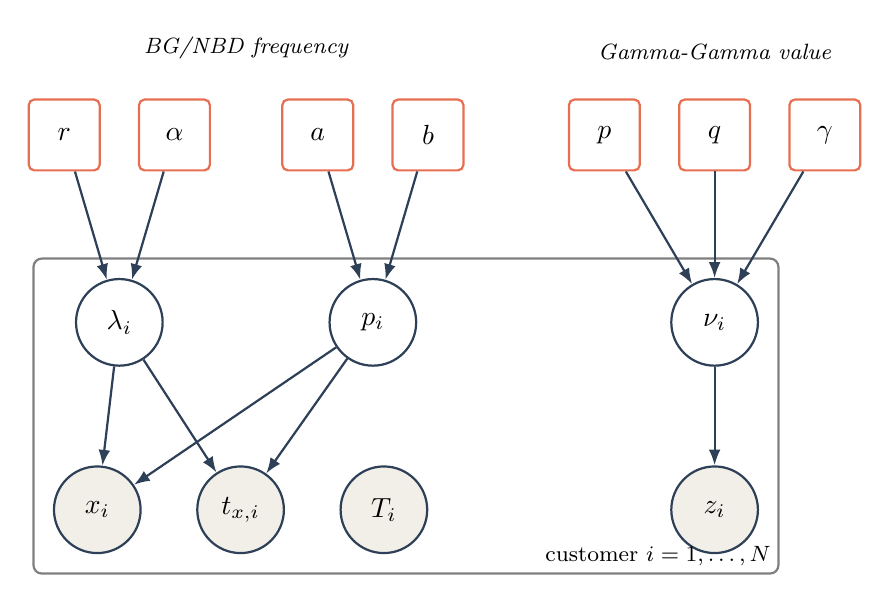
\begin{tikzpicture}[x=14mm, y=14mm]
    % ── Population-level hyperparameters (rectangles) ────────────
    \node[hyper] (r)     at (0.0, 0) {$r$};
    \node[hyper] (alpha) at (1.0, 0) {$\alpha$};
    \node[hyper] (a)     at (2.3, 0) {$a$};
    \node[hyper] (b)     at (3.3, 0) {$b$};
    \node[hyper] (pg)    at (4.9, 0) {$p$};
    \node[hyper] (q)     at (5.9, 0) {$q$};
    \node[hyper] (g)     at (6.9, 0) {$\gamma$};

    \node[font=\footnotesize\itshape, anchor=south] at (1.65,0.6) {BG/NBD frequency};
    \node[font=\footnotesize\itshape, anchor=south] at (2.8,0.6) {};
    \node[font=\footnotesize\itshape, anchor=south] at (5.9,0.6) {Gamma-Gamma value};

    % ── Latent per-customer parameters (open circles) ───────────
    \node[latent] (lambda) at (0.5, -1.7) {$\lambda_i$};
    \node[latent] (pdrop)  at (2.8, -1.7) {$p_i$};
    \node[latent] (nu)     at (5.9, -1.7) {$\nu_i$};

    % ── Observed data (shaded circles) ──────────────────────────
    \node[obs] (x)  at (0.3, -3.4) {$x_i$};
    \node[obs] (tx) at (1.6, -3.4) {$t_{x,i}$};
    \node[obs] (T)  at (2.9, -3.4) {$T_i$};
    \node[obs] (z)  at (5.9, -3.4) {$z_i$};

    % ── Edges ───────────────────────────────────────────────────
    \draw[conn] (r) -- (lambda);      \draw[conn] (alpha) -- (lambda);
    \draw[conn] (a) -- (pdrop);       \draw[conn] (b) -- (pdrop);
    \draw[conn] (pg) -- (nu);         \draw[conn] (q) -- (nu);   \draw[conn] (g) -- (nu);
    \draw[conn] (lambda) -- (x);      \draw[conn] (lambda) -- (tx);
    \draw[conn] (pdrop) -- (x);       \draw[conn] (pdrop) -- (tx);
    \draw[conn] (nu) -- (z);

    % ── Plate over customers ────────────────────────────────────
    \begin{scope}[on background layer]
      \node[plate, fit=(lambda)(pdrop)(nu)(x)(tx)(T)(z)] (plate) {};
    \end{scope}
    \node[anchor=south east, font=\footnotesize, inner sep=3pt]
      at (plate.south east) {customer $i = 1,\dots,N$};
  \end{tikzpicture}
  \caption[Graphical model of the BG/NBD + Gamma-Gamma framework]{Plate representation of the joint BG/NBD~$+$~Gamma-Gamma model. Rounded rectangles are population-level hyperparameters; open circles are latent per-customer parameters (transaction rate $\lambda_i$, dropout probability $p_i$, spend rate $\nu_i$); shaded circles are observed data (repeat purchases $x_i$, recency $t_{x,i}$, observation window $T_i$, average value $z_i$). The plate denotes replication over all $N$ customers.}
  \label{fig:bgnbd-plate}
\end{figure}


% Buy-till-you-die timeline for a single customer
\begin{figure}[htbp]
  \centering
  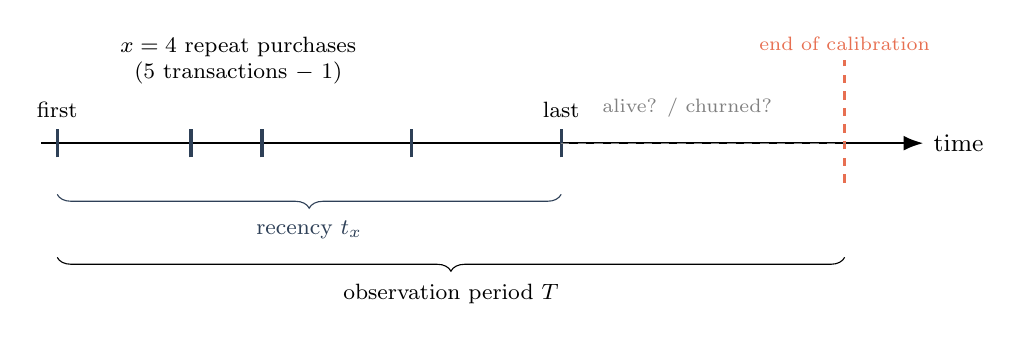
\begin{tikzpicture}[x=1cm, y=1cm]
    % time axis
    \draw[-{Latex[length=2.5mm]}, thick] (-0.2,0) -- (11,0) node[right, font=\small] {time};

    % observed purchases (ticks)
    \foreach \px in {0, 1.7, 2.6, 4.5, 6.4}{
      \draw[bayesblue, very thick] (\px,-0.18) -- (\px,0.18);
    }
    \node[above, font=\footnotesize] at (0,0.2)   {first};
    \node[above, font=\footnotesize] at (6.4,0.2) {last};

    % observation end
    \draw[accentorange, very thick, dashed] (10,-0.5) -- (10,1.05);
    \node[above, font=\scriptsize, accentorange] at (10,1.05) {end of calibration};

    % unobserved-after-last region
    \draw[gray, dashed] (6.4,0) -- (10,0);
    \node[font=\scriptsize, align=center, gray] at (8.0,0.45) {alive? / churned?};

    % brace: recency t_x (first -> last)
    \draw[decorate, decoration={brace, amplitude=5pt, mirror}, bayesblue]
      (0,-0.65) -- (6.4,-0.65)
      node[midway, below=6pt, font=\footnotesize, bayesblue] {recency $t_x$};

    % brace: observation period T (first -> end)
    \draw[decorate, decoration={brace, amplitude=5pt, mirror}, black]
      (0,-1.45) -- (10,-1.45)
      node[midway, below=6pt, font=\footnotesize] {observation period $T$};

    % frequency annotation
    \node[font=\footnotesize, align=center] at (2.3,1.05)
      {$x = 4$ repeat purchases\\ (5 transactions $-$ 1)};
  \end{tikzpicture}
  \caption[Buy-till-you-die timeline]{The buy-till-you-die logic for one customer. Five transactions are observed; the model summarises them as frequency $x$, recency $t_x$, and observation window $T$. After the last purchase the customer's state is latent: the BG/NBD model infers $P(\text{alive})$ from how recently and how often they bought relative to $T$.}
  \label{fig:btyd-timeline}
\end{figure}


\subsection{Key Model Outputs}
\label{sec:bgnbd-outputs}

Given a customer's observed history, summarised by frequency $x$ (number of repeat transactions), recency $t_x$ (time of last purchase), and observation period $T$, the BG/NBD model provides:

\begin{itemize}
  \item \textbf{$P(\text{alive})$.} The posterior probability that a customer remains active at the end of the observation period, directly addressing the latent-attrition challenge inherent in non-contractual CLV estimation.
  \item \textbf{Conditional expected transactions.} $E[X(t) \mid x, t_x, T]$ denotes the expected number of purchases over a future period of length $t$, based on the customer's history. This output constitutes the transaction-count component of CLV.
\end{itemize}

Both outputs are computed as expectations over the posterior distributions of individual customer parameters, naturally integrating uncertainty about each customer's true transaction frequency and dropout probability. Figure~\ref{fig:recency-T} previews the empirical $(\text{recency}, T)$ structure of the UCI Online Retail II calibration sample that these quantities are derived from.

\condfig{../outputs/eda/08_recency_vs_T.png}{0.62\linewidth}{Empirical recency versus observation period ($T$) for the calibration sample. Every customer necessarily lies on or below the diagonal $\text{recency} = T$; the spread of points away from the diagonal encodes the latent-activity signal the BG/NBD model exploits.}{fig:recency-T}

\subsection{Model Assumptions and Limitations}
\label{sec:bgnbd-assumptions}

The BG/NBD model relies on several underlying assumptions:

\begin{itemize}
  \item \textbf{Stationarity.} Each customer's transaction rate $\lambda$ and dropout probability $p$ are assumed constant over time. Real-world behaviour can shift owing to lifecycle progression, marketing activity, or broader market trends.
  \item \textbf{Independence of purchase and dropout.} The framework presumes no relationship between how frequently a customer purchases and their likelihood of churning. In practice, highly engaged customers may display distinct attrition patterns.
  \item \textbf{Absence of covariates.} The standard model excludes customer-level factors such as demographics, acquisition source, or marketing exposure. The hierarchical extensions of Section~\ref{sec:hierarchical} partially mitigate this by allowing segment-level variation.
\end{itemize}

Despite these simplifications, the BG/NBD model has consistently performed well in empirical validation studies and remains the predominant probabilistic approach for analysing non-contractual customer populations \parencite{fader2009}.

\section{The Gamma-Gamma Model for Monetary Value}
\label{sec:gg}

The BG/NBD model predicts the number of future transactions but does not model their value. The Gamma-Gamma model, introduced by \textcite{fader2013}, complements the BG/NBD by modelling the monetary value of individual transactions, enabling complete CLV estimation when combined with the transaction-count predictions.

\subsection{Model Specification}
\label{sec:gg-spec}

The Gamma-Gamma model assumes the following generative process:

\begin{itemize}
  \item \textbf{Individual spending.} Each customer's average transaction value $z$ follows a Gamma distribution, $z \mid p, \nu \sim \text{Gamma}(p, \nu)$, where $\nu$ is individual-specific.
  \item \textbf{Heterogeneity across customers.} The individual-specific rate $\nu$ varies across customers according to another Gamma distribution, $\nu \sim \text{Gamma}(q, \gamma)$.
\end{itemize}

This structure produces a marginal distribution for average transaction values that accommodates the right-skewed spending distributions typically observed in retail data. The model's three parameters $(p, q, \gamma)$ are estimated at the population level.

\subsection{Key Assumption: Independence of Frequency and Monetary Value}
\label{sec:gg-independence}

A critical assumption of the Gamma-Gamma model is that there is no systematic relationship between a customer's purchase frequency and their average transaction value. This is necessary for the monetary and frequency components of CLV to be modelled independently and combined multiplicatively. In practice the assumption should be verified empirically by computing the correlation between purchase frequency and average transaction value in the calibration data (Figure~\ref{fig:rfm-corr}). Violation can lead to biased CLV estimates, and the empirical analysis explicitly tests this condition.

\condfig{../outputs/eda/10_rfm_correlation.png}{0.7\linewidth}{Correlation structure among the RFM summary statistics in the calibration data. The frequency--monetary association is the quantity that must be near zero for the Gamma-Gamma independence assumption to hold.}{fig:rfm-corr}

\subsection{CLV Computation}
\label{sec:gg-clv}

With both models estimated, individual-level CLV over a future horizon of $t$ periods is computed as

\begin{equation}
  \text{CLV}_i = \underbrace{E\big[\text{transactions}_i(t)\big]}_{\text{BG/NBD}} \times \underbrace{E\big[\text{monetary}_i\big]}_{\text{Gamma-Gamma}} \times \text{margin factor}.
  \label{eq:clv-product}
\end{equation}

In the Bayesian formulation, both the expected transaction count and the expected monetary value are posterior distributions rather than point estimates. CLV is therefore itself a posterior distribution, enabling probabilistic statements such as ``there is a 90\% probability that this customer's 12-month CLV lies between \$150 and \$420.'' This distributional CLV is the foundation for the decision-theoretic targeting framework of Section~\ref{sec:decision}.

\section{Hierarchical Extensions: Partial Pooling Across Segments}
\label{sec:hierarchical}

The standard BG/NBD and Gamma-Gamma models estimate a single set of population-level parameters for the entire customer base, implicitly assuming all customers are drawn from the same behavioural distribution. In practice, meaningful differences may exist across segments, for example, customers in different countries, acquisition channels, or product categories. Hierarchical (multilevel) Bayesian models address this by introducing segment-level parameters that are themselves drawn from a shared hyperprior. This produces \emph{partial pooling}: segment-level estimates are pulled toward the global mean in proportion to their uncertainty, borrowing statistical strength from data-rich segments to stabilise estimates for data-sparse ones \parencite{gelmanhill2006}. Figure~\ref{fig:hierarchy} depicts this structure.

% Hierarchical partial-pooling structure
\begin{figure}[htbp]
  \centering
  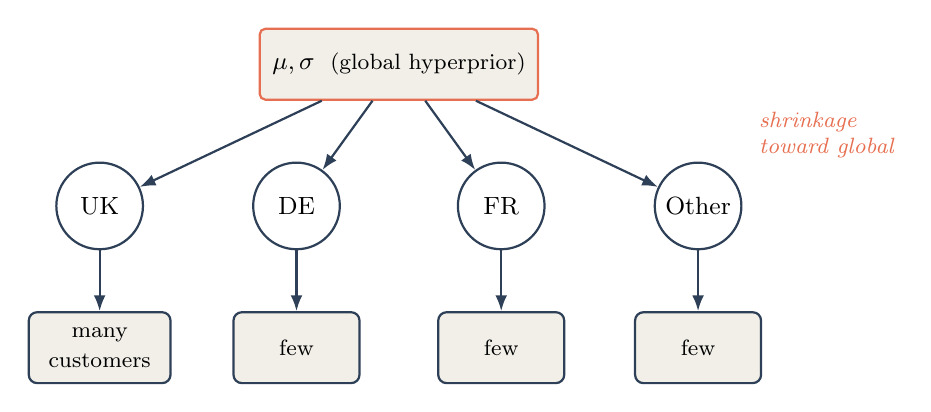
\begin{tikzpicture}[x=1cm, y=1cm, every node/.style={font=\small}]
    % global hyperprior
    \node[hyper, fill=softgray] (global) at (5,3)
      {\,$\mu,\sigma$ \;\footnotesize(global hyperprior)\,};

    % segment-level parameters
    \node[latent] (uk) at (1.2,1.2) {UK};
    \node[latent] (de) at (3.7,1.2) {DE};
    \node[latent] (fr) at (6.3,1.2) {FR};
    \node[latent] (ot) at (8.8,1.2) {Other};

    % customers
    \node[box, minimum width=18mm] (cuk) at (1.2,-0.6) {\footnotesize many\\\footnotesize customers};
    \node[box, minimum width=16mm] (cde) at (3.7,-0.6) {\footnotesize few};
    \node[box, minimum width=16mm] (cfr) at (6.3,-0.6) {\footnotesize few};
    \node[box, minimum width=16mm] (cot) at (8.8,-0.6) {\footnotesize few};

    % edges: global -> segments (partial pooling)
    \draw[conn] (global) -- (uk);
    \draw[conn] (global) -- (de);
    \draw[conn] (global) -- (fr);
    \draw[conn] (global) -- (ot);

    % edges: segments -> customers
    \draw[conn] (uk) -- (cuk);
    \draw[conn] (de) -- (cde);
    \draw[conn] (fr) -- (cfr);
    \draw[conn] (ot) -- (cot);

    % shrinkage annotation
    \node[font=\footnotesize\itshape, accentorange, align=left, anchor=west] at (9.4,2.1)
      {\,shrinkage\\ \,toward global};
  \end{tikzpicture}
  \caption[Hierarchical partial pooling]{Hierarchical (partial-pooling) structure across country segments. Each segment's behavioural parameters are drawn from a shared global hyperprior, so estimates for data-sparse segments (DE, FR, Other) are pulled toward the global mean, borrowing strength from the data-rich UK segment. Complete pooling would collapse the middle layer; no pooling would remove the global hyperprior entirely.}
  \label{fig:hierarchy}
\end{figure}


\subsection{Partial Pooling vs.\ Alternatives}
\label{sec:pooling}

Three estimation strategies exist for multi-segment data, summarised in Table~\ref{tab:pooling}.

\begin{table}[htbp]
  \centering
  \caption{Estimation strategies for multi-segment customer data.}
  \label{tab:pooling}
  \begin{tabularx}{\linewidth}{@{}l Y Y@{}}
    \toprule
    \textbf{Strategy} & \textbf{Approach} & \textbf{Limitation} \\
    \midrule
    Complete pooling & Ignore segment structure; estimate one global model & Ignores real differences between segments \\
    \addlinespace
    No pooling & Estimate fully independent models per segment & Noisy estimates for small segments; no information sharing \\
    \addlinespace
    Partial pooling & Hierarchical model; segment parameters drawn from a shared prior & More complex to implement; requires careful prior specification \\
    \bottomrule
  \end{tabularx}
\end{table}

The UCI Online Retail II dataset contains customers from multiple countries (UK, Germany, France, Netherlands, among others), with the UK accounting for the majority of transactions and other markets contributing substantially fewer observations (Figure~\ref{fig:country}). This creates an ideal testing ground for hierarchical modelling: the UK segment provides abundant data to estimate behavioural parameters precisely, while smaller country segments benefit from partial pooling that borrows strength from the global estimate. RQ2 directly tests whether this hierarchical structure improves CLV prediction for data-sparse segments.

\condfig{../outputs/eda/11_country_customers.png}{0.72\linewidth}{Customer counts by country segment in the calibration data. The pronounced imbalance, a dominant UK segment alongside several small markets, is precisely the regime in which partial pooling is expected to help.}{fig:country}

\subsection{Implementation Considerations}
\label{sec:noncentered}

Hierarchical models introduce additional computational challenges. The \emph{centred} parameterisation, in which segment parameters are drawn directly from the hyperprior, can create pathological posterior geometries known as Neal's funnel \parencite{neal2003}. These geometries cause MCMC samplers to explore inefficiently, producing low effective sample sizes and divergent transitions. The standard solution is the \emph{non-centred} parameterisation, which reparameterises the model so that the sampler operates on standardised (unit-normal) variables that are then scaled and shifted by the hyperparameters. This breaks the problematic correlation structure and typically resolves funnel-related sampling difficulties. The empirical implementation employs non-centred parameterisation where diagnostics indicate it is necessary.

\section{Decision Theory Under Uncertainty}
\label{sec:decision}

A distinctive advantage of Bayesian CLV models is that they produce full posterior distributions over customer-level CLV, enabling principled decision-making under uncertainty. This section introduces the decision-theoretic framework that RQ3 evaluates empirically.

\subsection{The Targeting Problem}
\label{sec:targeting}

Consider a retention campaign with a fixed per-customer cost $c$. The firm must decide which customers to target. Under a point-estimate approach, the decision rule is typically: target all customers whose estimated CLV exceeds $c$. This ignores the uncertainty around the estimate; a customer with a CLV point estimate of \$100 and a cost threshold of \$90 is treated identically regardless of whether the 90\% credible interval is $[\$95, \$105]$ (high confidence) or $[\$20, \$180]$ (low confidence).

Under a Bayesian decision-theoretic framework, the targeting decision instead uses the full posterior. The optimal decision for each customer depends on the posterior probability that their CLV exceeds the cost threshold:

\begin{equation}
  \text{Target customer } i \quad\text{if}\quad P(\text{CLV}_i > c \mid \text{data}) > \tau,
  \label{eq:decision-rule}
\end{equation}

where $\tau$ is a probability threshold chosen by the firm to balance the cost of false positives (targeting customers who would not generate sufficient value) against the cost of false negatives (missing valuable customers). This framework naturally accounts for estimation uncertainty and can be tuned to the firm's risk appetite. Figure~\ref{fig:decision} contrasts two customers with the same posterior mean but different uncertainty, illustrating why the probabilistic rule can differ from the point-estimate rule.

% Decision theory: two posteriors, same mean, different uncertainty
\begin{figure}[htbp]
  \centering
  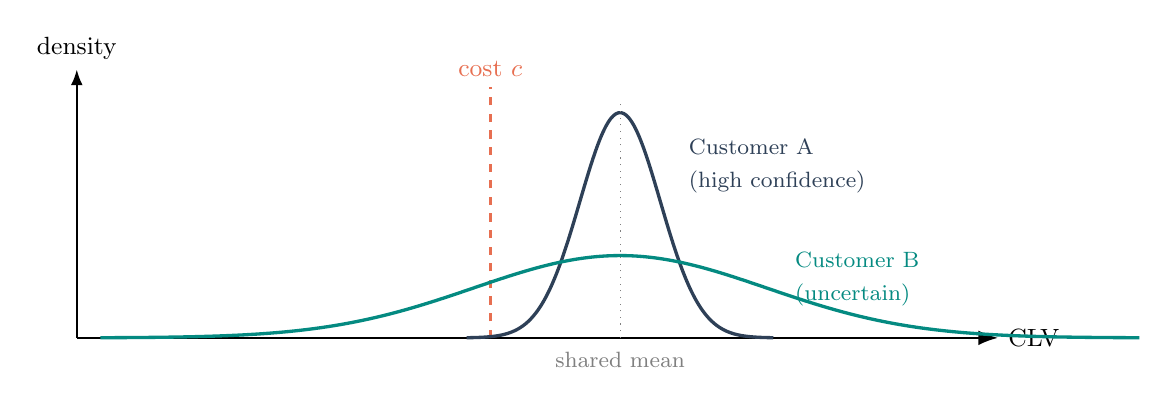
\begin{tikzpicture}[x=3cm, y=1.1cm]
    % axes
    \draw[-{Latex[length=2.5mm]}, thick] (-1.3,0) -- (2.6,0)
      node[right, font=\small] {CLV};
    \draw[-{Latex[length=2mm]}, thick] (-1.3,0) -- (-1.3,3.1)
      node[above, font=\small] {density};

    % cost threshold c
    \draw[accentorange, very thick, dashed] (0.45,0) -- (0.45,2.9);
    \node[accentorange, font=\small, anchor=south] at (0.45,2.9) {cost $c$};

    % Customer A: narrow, high-confidence (mostly above c)
    \draw[bayesblue, very thick, domain=0.35:1.65, samples=120, smooth]
      plot (\x, {2.6*exp(-((\x-1.0)^2)/(2*0.17*0.17))});
    \node[bayesblue, font=\footnotesize, anchor=west] at (1.25,2.2) {Customer A};
    \node[bayesblue, font=\footnotesize, anchor=west] at (1.25,1.8) {(high confidence)};

    % Customer B: wide, uncertain (straddles c)
    \draw[tealgreen, very thick, domain=-1.2:3.2, samples=160, smooth]
      plot (\x, {0.95*exp(-((\x-1.0)^2)/(2*0.62*0.62))});
    \node[tealgreen, font=\footnotesize, anchor=west] at (1.7,0.9) {Customer B};
    \node[tealgreen, font=\footnotesize, anchor=west] at (1.7,0.5) {(uncertain)};

    % shared mean marker
    \draw[gray, dotted] (1.0,0) -- (1.0,2.7);
    \node[gray, font=\footnotesize, anchor=north] at (1.0,-0.05) {shared mean};
  \end{tikzpicture}
  \caption[Decision theory under uncertainty]{Two customers with the \emph{same} posterior-mean CLV but different uncertainty. A point-estimate rule treats them identically. The decision-theoretic rule targets customer $i$ when $P(\text{CLV}_i > c) > \tau$: customer A places almost all posterior mass above the cost $c$ and is a confident target, whereas customer B's mass straddles $c$, so the probabilistic rule appropriately discounts the apparent value.}
  \label{fig:decision}
\end{figure}


\subsection{Expected Improvement Over Point Estimates}
\label{sec:improvement}

The decision-theoretic approach is expected to outperform point-estimate targeting in two specific scenarios:

\begin{itemize}
  \item \textbf{High-uncertainty customers near the threshold.} Customers whose posterior CLV distribution spans the cost threshold benefit most from the probabilistic treatment. Point estimates arbitrarily classify them as above or below the threshold, while the posterior probability provides a calibrated measure of confidence.
  \item \textbf{Data-sparse segments.} Customers with limited purchase history have wider posterior distributions. The decision-theoretic framework naturally expresses this uncertainty, preventing overconfident targeting of customers whose apparent high value may be driven by sampling noise.
\end{itemize}

The empirical analysis tests whether these expected improvements materialise on the UCI Online Retail II holdout data.

\section{Summary of Theoretical Findings and Hypotheses}
\label{sec:hypotheses}

This chapter has established the Bayesian probabilistic framework for CLV prediction. The key theoretical findings are:

\begin{itemize}
  \item The BG/NBD~$+$~Gamma-Gamma framework provides a complete generative model for non-contractual CLV that jointly captures purchase timing, latent attrition, and monetary value, producing full posterior distributions over individual-level CLV.
  \item Hierarchical extensions enable partial pooling across segments, which theory predicts will improve estimates for data-sparse segments by borrowing strength from data-rich ones.
  \item Decision-theoretic targeting using posterior CLV distributions provides a principled framework for risk-aware customer selection that should outperform point-estimate approaches, particularly for high-uncertainty customers near the targeting threshold.
\end{itemize}

These findings generate three testable hypotheses for the empirical analysis, collected in Table~\ref{tab:hypotheses}.

\begin{table}[htbp]
  \centering
  \caption{Testable hypotheses evaluated in the empirical analysis.}
  \label{tab:hypotheses}
  \begin{tabularx}{\linewidth}{@{}p{1.1cm} Y@{}}
    \toprule
    \textbf{ID} & \textbf{Hypothesis} \\
    \midrule
    H1 & The Bayesian BG/NBD~$+$~Gamma-Gamma model will achieve competitive or superior out-of-sample accuracy compared to RFM-heuristic and XGBoost baselines, with the additional benefit of calibrated uncertainty estimates. \\
    \addlinespace
    H2 & Hierarchical partial pooling across country segments will reduce prediction error for small-market customers (e.g., Germany, France) compared to both complete-pooling and no-pooling alternatives. \\
    \addlinespace
    H3 & Decision-theoretic targeting using $P(\text{CLV} > c)$ will produce higher cumulative realised value than targeting based on point-estimate CLV rankings. \\
    \bottomrule
  \end{tabularx}
\end{table}

% ============================================================
% CHAPTER 4 — METHODOLOGY
% ============================================================
% ============================================================
% CHAPTER 4 — METHODOLOGY
% ============================================================
\chapter{Methodology}
\label{ch:methodology}

This chapter describes the empirical strategy used to evaluate the three hypotheses of Section~\ref{sec:hypotheses}. It specifies the research design, the dataset and its preparation, the Bayesian and baseline models, the inference procedure, and the evaluation protocol that links each metric to a hypothesis.

\section{Research Design}
\label{sec:design}

The study adopts a \emph{calibration--holdout} predictive-validation design, the standard protocol for customer-base analysis \parencite{fader2005}. The transaction history is split chronologically at a fixed cut-off date: data before the cut-off (the \emph{calibration} period) are used to estimate every model, and data after it (the \emph{holdout} period) provide the ground truth against which predictions are scored. Because the split is temporal rather than random, the design measures genuine forecasting performance and precludes information leakage from the future into model fitting.

All models are trained on identical calibration inputs and evaluated on identical holdout targets, so differences in performance are attributable to the models rather than to the data partition. The design instruments each research question with a dedicated component, completing the gap--hypothesis--method chain of Section~\ref{sec:research-gap}: Gap~1/RQ1 through the accuracy and uncertainty-calibration protocol (coverage, CRPS; Section~\ref{sec:evaluation}); Gap~2/RQ2 through the three-way pooling comparison and per-segment error analysis (Section~\ref{sec:specification}); and Gap~3/RQ3 through the realised-value targeting simulation (Section~\ref{sec:evaluation}).

\section{Dataset}
\label{sec:dataset}

The empirical analysis uses the UCI \emph{Online Retail II} dataset, a transaction-level record of a UK-based online retailer spanning 1~December~2009 to 9~December~2011. The raw data comprise \num{1{,}067{,}371} line items across two annual sheets, with fields for invoice number, stock code, description, quantity, unit price, invoice timestamp, customer identifier, and country. The setting is non-contractual and episodic: customers purchase sporadically with no subscription, making activity status latent and the dataset an appropriate testbed for the probabilistic models of Chapter~\ref{ch:bayesian}.

\section{Data Preparation}
\label{sec:preparation}

\subsection{Cleaning}
\label{sec:cleaning}

The raw transactions are cleaned in five steps, implemented in \texttt{src/data.py}: (i) rows with a missing customer identifier are dropped, since customer-level modelling is impossible without them; (ii) cancellations, identified by invoice numbers beginning with ``C'', are removed; (iii) non-product stock codes representing operational charges (postage, bank charges, manual adjustments, and similar) are filtered out; (iv) rows with non-positive quantity or price are discarded; and (v) line-level revenue is computed as quantity~$\times$~price. Cleaning reduces the data from \num{1{,}067{,}371} to \num{802{,}679} line items, removing \SI{24.8}{\percent} of rows. Figure~\ref{fig:cleaning} visualises the attrition at each step.

\condfig{../outputs/eda/01_cleaning_waterfall.png}{0.8\linewidth}{Data-cleaning waterfall: the cumulative effect of each filtering step on the row count, from \num{1{,}067{,}371} raw line items to \num{802{,}679} retained transactions.}{fig:cleaning}

\subsection{Temporal Split}
\label{sec:split}

The cleaned data are partitioned at \texttt{CAL\_END}~$=$~1~March~2011. The calibration period (1~December~2009 to 28~February~2011, \num{473{,}386} transactions) yields a maximum customer observation window of \num{65.1} weeks; the holdout period (1~March~2011 to 9~December~2011, \num{329{,}293} transactions) spans \num{40.4} weeks and defines the prediction horizon over which forecasts are scored. Figure~\ref{fig:timeseries} shows the monthly revenue series and the location of the split.

\condfig{../outputs/eda/04_monthly_timeseries.png}{0.85\linewidth}{Monthly transaction revenue across the full observation window. The calibration/holdout boundary is fixed at 1~March~2011.}{fig:timeseries}

\subsection{Customer-Level Aggregation}
\label{sec:aggregation}

Calibration transactions are collapsed to one row per customer, producing the summary statistics required by the BG/NBD and Gamma-Gamma models. Following the conventions of \textcite{fader2005} and \textcite{fader2013}:

\begin{itemize}
  \item \textbf{Frequency} ($x$) is the number of \emph{repeat} purchases, i.e.\ the count of purchase occasions minus one. One-time buyers have $x = 0$.
  \item \textbf{Recency} ($t_x$) is the time, in weeks, from a customer's first to their last purchase.
  \item \textbf{$T$} is the time, in weeks, from the first purchase to the end of the calibration period.
  \item \textbf{Monetary value} ($m$) is the mean revenue per repeat transaction; the first purchase is excluded, per the Gamma-Gamma convention, and one-time buyers are assigned $m = 0$.
\end{itemize}

Aggregation yields \num{4{,}522} customers, of whom \SI{67.0}{\percent} are repeat purchasers and \SI{33.0}{\percent} are one-time buyers. The mean repeat-purchase frequency is \num{3.78} (median~1, maximum~200), reflecting the heavy right skew typical of retail. Among repeat purchasers, the mean value per transaction is \pounds\num{384.99} (median \pounds\num{298.52}). Time is expressed in weeks throughout (\texttt{time\_unit~=~"W"}).

\subsection{Country Segmentation}
\label{sec:segmentation}

To support the hierarchical analysis (RQ2), customers are labelled by country. Countries with fewer than \num{30} customers are collapsed into an ``Other'' segment to avoid unstable per-segment estimates, yielding four segments: United Kingdom (\num{4{,}152} customers), Other (\num{242}), Germany (\num{74}), and France (\num{54}). The pronounced imbalance (the UK accounts for over \SI{91}{\percent} of customers) is exactly the regime in which partial pooling is expected to help the small segments (Figure~\ref{fig:country}).

\section{Exploratory Findings}
\label{sec:eda}

Before modelling, the calibration sample is examined to characterise the input distributions and to test a key modelling assumption. The frequency distribution (Figure~\ref{fig:freqdist}) is heavily right-skewed, with most customers making few repeat purchases and a long tail of highly active buyers. The monetary distribution (Figure~\ref{fig:monetarydist}) is similarly right-skewed, motivating the Gamma-Gamma model's accommodation of skewed spend.

\condfig{../outputs/eda/06_rfm_frequency.png}{0.7\linewidth}{Distribution of repeat-purchase frequency in the calibration sample. The mass at low frequencies and the long right tail are characteristic of non-contractual retail.}{fig:freqdist}

\condfig{../outputs/eda/09_rfm_monetary.png}{0.7\linewidth}{Distribution of average transaction value among repeat purchasers. The right skew motivates the Gamma-Gamma specification.}{fig:monetarydist}

\paragraph{Test of the Gamma-Gamma independence assumption.}
The Gamma-Gamma model requires that purchase frequency and average transaction value be independent (Section~\ref{sec:gg-independence}). Empirically, the correlation between frequency and monetary value among repeat purchasers is weak: Pearson $r = 0.13$ and Spearman $\rho = 0.21$ (Figure~\ref{fig:rfm-corr}). The association is small enough that the independence assumption is approximately satisfied, but the mildly positive sign indicates that more frequent buyers spend slightly more per order; this caveat is revisited when interpreting the monetary-model results and in the limitations (Section~\ref{sec:limitations}).

\section{Model Specification}
\label{sec:specification}

Three Bayesian models are implemented in PyMC (\texttt{src/models.py}), following the generative structure of Chapter~\ref{ch:bayesian}.

\paragraph{Pooled BG/NBD.}
The standard BG/NBD model \parencite{fader2005} is estimated using the \texttt{pymc-marketing} implementation, which expresses the likelihood in the numerically stable form of \textcite{fader2005} (their expression~4). This form avoids the underflow and the ill-conditioned posterior geometry that a naive coding of the two-branch likelihood produces, and it samples efficiently. The population parameters $r, \alpha, a, b$ are assigned weakly informative half-normal priors whose scales are set from summary statistics of the calibration data (\texttt{src/priors.py}), which places prior mass in the region the data support and further stabilises sampling. The latent per-customer transaction rate and dropout probability are integrated out analytically, so the sampler operates only on the four population parameters.

\paragraph{Hierarchical BG/NBD.}
The hierarchical variant is a custom PyMC model that reuses the same stable likelihood but places the four BG/NBD parameters at the country-segment level, each drawn from a shared hyperprior. To avoid the funnel geometry described in Section~\ref{sec:noncentered}, a non-centred parameterisation is used: standardised normal offsets $z \sim \text{Normal}(0,1)$ per segment are scaled and shifted by the hyperparameters and mapped to the positive reals through an exponential (log-normal) link. A deliberately tight between-segment scale prior controls the residual funnel induced by the small country segments. This yields segment-specific $(r, \alpha, a, b)$ while permitting partial pooling toward the global mean.

\paragraph{Gamma-Gamma.}
The Gamma-Gamma monetary model \parencite{fader2013} is estimated with the corresponding \texttt{pymc-marketing} implementation, fitted only on repeat purchasers ($x > 0$), since average transaction value is undefined for one-time buyers. Its three population parameters receive half-normal priors, and expected spend is obtained from the model's posterior. CLV for one-time buyers imputes the population mean spend.

\section{Bayesian Inference}
\label{sec:inference}

All posteriors are obtained by Hamiltonian Monte Carlo using the No-U-Turn Sampler (Section~\ref{sec:mcmc}). Each model is sampled with \num{4} chains of \num{1000} draws following \num{1000} tuning iterations and a fixed random seed of \num{42} for reproducibility. The target acceptance probability is \num{0.9} for the pooled and Gamma-Gamma models and is raised to \num{0.95} for the hierarchical model to control its sharper posterior geometry. Convergence is assessed with the diagnostics of Section~\ref{sec:mcmc}: split-$\widehat{R}$ (convergence requires values below \num{1.01}), effective sample size, the number of divergent transitions, and the Bayesian fraction of missing information. These diagnostics are reported in Section~\ref{sec:results-diagnostics} and determine whether reparameterisation was required for the hierarchical model.

\section{Baseline Models}
\label{sec:baselines}

Four non-Bayesian baselines (\texttt{src/baselines.py}) contextualise the probabilistic models:

\begin{itemize}
  \item \textbf{Naive (mean).} Predicts the population-average purchase rate and average spend for every customer; a lower bound on useful performance.
  \item \textbf{RFM heuristic.} Scores customers into quintiles on recency, frequency, and monetary value, and projects future transactions from a composite score scaled by the base purchase rate.
  \item \textbf{XGBoost (two-stage).} Gradient-boosted trees trained on engineered features (core RFM, derived ratios, inter-purchase-time statistics, and day-of-week/spend-trend temporal features), with separate models for the holdout transaction count and per-transaction spend, combined multiplicatively into CLV. This mirrors the BG/NBD~$+$~Gamma-Gamma decomposition, making the Bayesian-versus-ML comparison clean.
  \item \textbf{Pareto/NBD (optional).} The maximum-likelihood predecessor to BG/NBD, included where the \texttt{lifetimes} library is available.
\end{itemize}

\section{Prediction}
\label{sec:prediction}

For the Bayesian models, predictions are computed as expectations over the posterior. For each posterior draw, the conditional expected number of transactions over the holdout horizon, $E[X(t) \mid x, t_x, T]$, and the probability of being alive, $P(\text{alive})$, are evaluated for every customer; the Gamma-Gamma posterior yields the expected per-transaction value. Customer-level CLV is the product of the expected transaction count and expected value (Equation~\ref{eq:clv-product}). Because the computation is performed per draw, every prediction is itself a posterior distribution, from which means and credible intervals are derived. For quantities concerning \emph{realised} outcomes, namely predictive intervals and the targeting probability $P(\text{CLV} > c)$, the sampling variability of the outcome is added by drawing counts from the conditional predictive distribution per posterior draw, yielding the posterior predictive distribution; the distinction between the posterior of an expectation and the posterior predictive proves consequential in Sections~\ref{sec:results-uncertainty} and~\ref{sec:results-h3}.

\section{Evaluation Protocol}
\label{sec:evaluation}

Models are scored on the holdout period using a suite of metrics (\texttt{src/evaluation.py}), each mapped to a hypothesis (Table~\ref{tab:metric-map}).

\begin{table}[htbp]
  \centering
  \caption{Mapping of evaluation metrics to research hypotheses.}
  \label{tab:metric-map}
  \begin{tabularx}{\linewidth}{@{}l Y@{}}
    \toprule
    \textbf{Hypothesis} & \textbf{Metrics} \\
    \midrule
    H1 (accuracy + uncertainty) & MAE, RMSE, MAPE for transactions and CLV; Spearman and Gini for ranking; NDCG@$k$; credible-interval coverage and mean interval width; CRPS; $P(\text{alive})$ AUC and Brier score; decile calibration tables \\
    \addlinespace
    H2 (hierarchical pooling) & Per-country MAE for each model; posterior shrinkage of segment parameters toward the global mean \\
    \addlinespace
    H3 (decision-theoretic targeting) & Cumulative realised net value under point-estimate, posterior-probability, and oracle targeting, swept over targeting depth and intervention cost; targeting lift \\
    \bottomrule
  \end{tabularx}
\end{table}

\paragraph{Accuracy and ranking.}
Mean absolute error and root mean squared error measure point accuracy for both holdout transactions and CLV; the Gini coefficient and Spearman correlation measure ranking quality, and NDCG@100 and NDCG@500 measure top-$k$ ranking relevant to targeting.

\paragraph{Uncertainty calibration.}
For the Bayesian models, credible-interval coverage compares the nominal and empirical coverage of posterior predictive intervals (well-calibrated intervals achieve coverage close to nominal), the mean interval width quantifies sharpness, and the continuous ranked probability score (CRPS) jointly rewards accuracy and calibration. These metrics operationalise the ``calibrated uncertainty'' claim of H1, which point-prediction baselines cannot satisfy.

\paragraph{Activity classification.}
$P(\text{alive})$ is evaluated as a binary classifier of holdout activity (a customer is active if they make at least one holdout purchase; \SI{59.0}{\percent} of customers, \num{2{,}670} of \num{4{,}522}, are active) using AUC and the Brier score.

\paragraph{Decision-theoretic targeting.}
For H3, a targeting simulation ranks customers by (i) posterior mean CLV, (ii) the probability $P(\text{CLV} > c)$ computed from the posterior \emph{predictive} distribution of realised CLV, and (iii) realised value (oracle), and reports the cumulative net value captured at targeting depths of $5$--$50\%$. The intervention cost $c$ is swept over $\{\pounds 100, \pounds 300, \pounds 600, \pounds 1{,}200, \pounds 2{,}000\}$, a grid scaled to the magnitude of realised customer value in the holdout, to ensure the conclusion is robust to the cost assumption; $\pounds 600$ is the headline case.

\section{Implementation and Reproducibility}
\label{sec:implementation}

The pipeline is implemented in Python using PyMC~5 for inference \parencite{salvatier2016}, the \texttt{pymc-marketing} library for the standard BG/NBD and Gamma-Gamma implementations \parencite{pymcmarketing2024}, ArviZ for posterior handling and diagnostics, scikit-learn and XGBoost for baselines, and Matplotlib for figures. The full analysis is orchestrated by \texttt{src/run\_all\_models.py}, which executes data preparation, MCMC sampling, prediction, evaluation, table generation, and plotting as a single reproducible sequence. All stochastic components use fixed seeds, posterior traces are serialised to NetCDF, and result tables are exported as both CSV and \LaTeX{} for direct inclusion in this document.


% ============================================================
% CHAPTER 5 — RESULTS
% ============================================================
% ============================================================
% CHAPTER 5 — RESULTS
% ============================================================
\chapter{Results}
\label{ch:results}

This chapter reports the empirical results of the calibration--holdout evaluation and tests the three hypotheses of Section~\ref{sec:hypotheses}. Section~\ref{sec:results-diagnostics} establishes that the MCMC inference is trustworthy; Sections~\ref{sec:results-h1}--\ref{sec:results-h3} address H1, H2, and H3 in turn; and Section~\ref{sec:results-summary} collates the verdicts.

\paragraph{Note on reproduction.}
The tables and figures in this chapter are produced by \texttt{src/\allowbreak run\_all\_models.py} and written to \texttt{outputs/\allowbreak results/} and \texttt{outputs/\allowbreak figures/}; all numeric values quoted in the prose are read directly from those generated tables. The standard BG/NBD and Gamma-Gamma models are estimated with the \texttt{pymc-marketing} implementation of the numerically stable Fader--Hardie likelihood, while the hierarchical model is a custom PyMC implementation of the same likelihood with partial pooling across country segments.

\section{MCMC Convergence and Diagnostics}
\label{sec:results-diagnostics}

Before interpreting any posterior, the quality of the sampling is verified using the diagnostics of Section~\ref{sec:mcmc}. Figure~\ref{fig:rhat} shows the split-$\widehat{R}$ values for the pooled BG/NBD, hierarchical BG/NBD, and Gamma-Gamma models. Convergence is indicated when all parameters satisfy $\widehat{R} < 1.01$; the effective sample sizes and the number of divergent transitions for each model are summarised below. The trace and pair plots (Figures~\ref{fig:trace} and~\ref{fig:pairs}) provide a visual check on mixing and posterior correlation structure.

\condfig{../outputs/figures/rhat_bgnbd_standard.png}{0.7\linewidth}{Split-$\widehat{R}$ convergence diagnostics for the pooled BG/NBD model. The dashed line marks the $1.01$ threshold.}{fig:rhat}

\condfig{../outputs/figures/trace_bgnbd_standard.png}{0.85\linewidth}{Posterior trace plots for the pooled BG/NBD population parameters $(r, \alpha, a, b)$. Well-mixed, stationary chains indicate reliable sampling.}{fig:trace}

\condfig{../outputs/figures/pairs_bgnbd.png}{0.75\linewidth}{Pairwise posterior marginals for the BG/NBD parameters, with divergences highlighted. Strong correlations would motivate reparameterisation.}{fig:pairs}

For the hierarchical model, a non-centred parameterisation (Section~\ref{sec:noncentered}) with a tight between-segment scale was adopted to control the funnel geometry that the small country segments induce; Figure~\ref{fig:rhat-hier} confirms that this resolved the sampling pathologies. Across all three models the maximum split-$\widehat{R}$ is $1.002$ and the minimum bulk effective sample size exceeds $1{,}100$, with no divergent transitions. The diagnostics therefore indicate that the reported posteriors are well converged and provide a sound basis for the inferences that follow.

\condfig{../outputs/figures/rhat_bgnbd_hierarchical.png}{0.7\linewidth}{Split-$\widehat{R}$ for the hierarchical BG/NBD model under the non-centred parameterisation.}{fig:rhat-hier}

\section{H1: Predictive Accuracy and Calibrated Uncertainty}
\label{sec:results-h1}

\subsection{Point and Ranking Accuracy}
\label{sec:results-accuracy}

Table~\ref{tab:metrics_comparison} reports the headline comparison across all models for both holdout transaction prediction and CLV, covering error (MAE, RMSE, MAPE), ranking (Spearman, Gini), and top-$k$ relevance (NDCG). H1 predicts that the Bayesian BG/NBD~$+$~Gamma-Gamma model is competitive with or superior to the RFM-heuristic and XGBoost baselines. The results show that the Bayesian model attains a transaction MAE of $1.74$ against $2.12$ for XGBoost and $2.33$ for the RFM heuristic, and a CLV Gini of $0.86$ (versus $0.80$ for XGBoost). The ranking metrics are the most decisive: the Bayesian model reaches an NDCG@100 of $0.91$ against $0.53$ for XGBoost, so it identifies the highest-value customers far more reliably than either baseline while also carrying the lowest CLV MAE (\pounds$847$ against \pounds$1{,}478$ for XGBoost). The size of this ranking gap warrants explanation, since a value near $0.9$ against one near $0.5$ is a large margin. Two factors combine to produce it. First, the generative model borrows strength across the customer base, so even customers with sparse histories receive a sensibly ordered value estimate, whereas the discriminative XGBoost, trained to minimise average error, is comparatively indifferent to the exact ordering within the small high-value tail that NDCG@100 rewards. Second, the leakage-safe design gives XGBoost a shorter effective training window (Section~\ref{sec:limitations-eval}), which handicaps precisely the top-of-ranking task; its accuracy on bulk error metrics (transaction MAE $2.12$) is much closer to the Bayesian model than the NDCG gap alone would suggest. The Bayesian model is thus superior, not merely competitive, on out-of-sample accuracy.

\resulttable{metrics_comparison}{Model comparison across transaction and CLV prediction metrics.}{tab:metrics_comparison}

The decile calibration plot (Figure~\ref{fig:calibration}) shows predicted versus actual transactions for each model. Points close to the diagonal indicate good calibration of the point predictions; systematic departure in the top deciles would signal over- or under-prediction for the most active customers.

\condfig{../outputs/figures/calibration_comparison.png}{0.95\linewidth}{Decile calibration: mean predicted versus mean actual holdout transactions for each model. The diagonal denotes perfect calibration.}{fig:calibration}

\subsection{The XGBoost Benchmark}
\label{sec:results-xgboost}

Because XGBoost is the strongest baseline, understanding \emph{why} it trails the Bayesian model is instructive. Figure~\ref{fig:xgb-importance} reports the gain-based feature importances of its transaction model. The ranking is dominated by \textbf{frequency} ($0.29$) and \textbf{purchase rate} ($0.16$), which together account for roughly $45\%$ of the total gain: given twenty-four engineered features, the model spends most of its explanatory power rediscovering the recency--frequency signal that the BG/NBD encodes structurally in its generative story. The remaining importance is spread thinly across the engineered rhythm features the parametric model cannot use, namely day-of-week purchase fractions and the mean and variability of inter-purchase times. That these behavioural extras add so little confirms that, on this dataset, the predictive content is concentrated in exactly the summaries the generative model already exploits.

\condfig{../outputs/figures/xgboost_feature_importance.png}{0.85\linewidth}{Gain-based feature importance of the XGBoost transaction model (top 12 of 24 features). Frequency and purchase rate dominate; the engineered day-of-week and inter-purchase-time features contribute comparatively little.}{fig:xgb-importance}

This explains the pattern in Table~\ref{tab:metrics_comparison}. XGBoost is genuinely competitive on bulk error: a transaction MAE of $2.12$ is far better than the naive and RFM baselines and within striking distance of the Bayesian model's $1.74$. Where it falls away sharply is at the top of the ranking, the regime that matters for targeting: its NDCG@100 is $0.53$ against $0.91$, and its CLV MAE is \pounds\num{1478} against \pounds\num{847}. Three factors combine to produce this gap. First, the squared-error objective optimises average accuracy, not the ordering of the sparse high-value tail that NDCG rewards. Second, the leakage-safe design trains it on a $21.4$-week inner window (Section~\ref{sec:xgboost}), a shorter supervision horizon than the full calibration window the Bayesian models use. Third, and most fundamentally, it has no mechanism to borrow strength across data-sparse customers and no native uncertainty, so it cannot express how confident any individual prediction is. XGBoost is thus the right benchmark precisely because it is a strong point predictor that nonetheless loses on the two axes, top-of-ranking accuracy and calibrated uncertainty, that motivate the Bayesian approach.

\subsection{Uncertainty Calibration}
\label{sec:results-uncertainty}

The distinctive claim of H1 is that the Bayesian model adds \emph{calibrated uncertainty} that point-prediction baselines cannot provide. Table~\ref{tab:coverage} reports the empirical coverage of posterior predictive credible intervals, the mean interval width, and the CRPS. Coverage close to the nominal level (e.g.\ empirical coverage near $90\%$ for the $90\%$ interval) indicates well-calibrated uncertainty; the observed coverage is $89.3\%$, almost exactly the nominal $90\%$, so the posterior predictive intervals are well calibrated. The posterior predictive distributions for a sample of customers (Figure~\ref{fig:postpred}) illustrate how the model expresses heterogeneous uncertainty across the customer base.

\resulttable{credible_interval_coverage}{Posterior predictive credible-interval coverage and CRPS.}{tab:coverage}

\condfig{../outputs/figures/posterior_predictive_bgnbd.png}{0.95\linewidth}{Posterior predictive distributions of holdout transactions for a sample of customers (violins), with realised values overlaid. The spread of each violin is the model's per-customer uncertainty.}{fig:postpred}

\subsection{Activity Prediction}
\label{sec:results-palive}

The $P(\text{alive})$ estimates are evaluated as a classifier of holdout activity (Table~\ref{tab:p_alive}). Because a customer with no repeat purchase is trivially assigned $P(\text{alive}) = 1$ under the BG/NBD model (they cannot have dropped out after a repeat that never occurred), the discrimination metrics are computed on repeat purchasers, for whom the estimate is informative. On this population the BG/NBD model achieves an AUC of $0.71$ and a Brier score of $0.21$, indicating moderate but useful discrimination of customers who remain active. An AUC of $0.71$ should be read as a genuine signal rather than a disappointing one: activity is a latent state that no model can observe, and a customer who is truly still active may simply not purchase again within the finite holdout window through ordinary randomness, which caps how well \emph{any} classifier can separate the two groups on this task. The value is well above the chance level of $0.5$, and, as the calibration-first framing of this thesis stresses, the probability is more useful for being calibrated than for being sharp. Figure~\ref{fig:palive} shows that $P(\text{alive})$ increases with calibration frequency, as theory predicts.

\resulttable{p_alive_evaluation}{$P(\text{alive})$ evaluation: binary activity-prediction metrics.}{tab:p_alive}

\condfig{../outputs/figures/p_alive_bgnbd_standard.png}{0.95\linewidth}{Distribution of $P(\text{alive})$ overall and by frequency group. Higher-frequency customers concentrate at higher $P(\text{alive})$.}{fig:palive}

\subsection{A Worked Example: One Customer End to End}
\label{sec:worked-example}

The aggregate metrics are best understood by watching the model reason about a single customer. Customer~14817, introduced in Section~\ref{sec:dist-data}, enters with only four numbers: frequency $x = 4$, recency $t_x = 33.1$ weeks, observation window $T = 49.2$ weeks, and mean repeat spend $m = \pounds 526$. From these the fitted model produces, in sequence, every quantity this thesis is concerned with.

First, activity. Despite the fifteen-week silence before the calibration cut-off, the pattern of four repeat purchases spread across the window yields $P(\text{alive}) = 0.88$: probably, but not certainly, still active. Second, future purchasing. The conditional expectation over the 40-week holdout horizon is $E[X] = 2.81$ transactions (90\% credible interval $[2.74, 2.88]$). Third, spend. The Gamma-Gamma model shrinks the customer's observed \pounds 526 toward the population mean, giving an expected value of roughly \pounds 485 per transaction. Multiplying the two components gives an expected CLV of \pounds\num{1364}, with a strikingly tight point-posterior interval of $[\pounds\num{1326}, \pounds\num{1401}]$.

That tight interval is where the worked example becomes instructive, because it reflects only \emph{parameter} uncertainty and is therefore the wrong interval for a decision about a realised outcome. The posterior \emph{predictive} distribution of the customer's actual holdout value, which additionally accounts for the sampling variability of the transaction count and the possibility of dropout, is far wider: a 90\% interval of $[\pounds 0, \pounds\num{2888})$, with substantial mass at zero (Figure~\ref{fig:worked}). The two distributions disagree sharply about the very question a targeting rule asks. At the headline intervention cost of \pounds 600, the probability $P(\text{CLV} > \pounds 600)$ computed from the posterior of the expectation is a falsely emphatic $1.00$, because the narrow spike sits entirely above the threshold; computed from the predictive distribution it is a candid $0.77$, acknowledging the roughly one-in-four chance the customer returns too little to justify the spend. This single customer previews the population-wide artefact examined in Section~\ref{sec:results-h3}. In the event, customer~14817 returned twice in the holdout and spent \pounds\num{1010}: profitable to target, above the cost, and comfortably inside the predictive interval that the point estimate's tight band would have hidden.

\condfig{../outputs/figures/worked_example_customer.png}{0.95\linewidth}{Two posteriors for one customer (ID~14817). The narrow posterior of $E[\text{CLV}]$ (orange) reflects parameter uncertainty only and lies entirely above the \pounds 600 cost, giving $P(\text{CLV}>\pounds 600)=1.00$. The posterior predictive of realised CLV (blue) is far wider, placing $\sim\!23\%$ of its mass below the cost, so the same probability computed correctly is $0.77$. The realised holdout value (\pounds\num{1010}) falls well inside the predictive distribution.}{fig:worked}

\paragraph{Verdict on H1.}
Taken together, the accuracy metrics (Table~\ref{tab:metrics_comparison}) and the uncertainty diagnostics (Table~\ref{tab:coverage}) indicate that H1 is supported: the Bayesian model is superior on accuracy, most clearly on the ranking metrics that matter for targeting, while uniquely providing well-calibrated predictive intervals.

\section{H2: Hierarchical Partial Pooling Across Segments}
\label{sec:results-h2}

H2 predicts that hierarchical partial pooling reduces prediction error for small country segments relative to the pooled (complete-pooling) model. The natural benchmark for this claim is the three-way comparison of \emph{complete} pooling, \emph{partial} pooling, and \emph{no} pooling, the last being an independent BG/NBD fitted separately on each segment. Table~\ref{tab:country_mae} reports per-country transaction MAE for all three specifications alongside the classical baselines, and Figure~\ref{fig:country-mae} visualises the comparison.

Two contrasts matter. Against complete pooling, the hierarchical model does not reduce error in the small markets: for Germany ($n=74$) its MAE is $1.635$ versus $1.622$, and for France ($n=54$) $2.318$ versus $2.223$, in both cases a marginal increase. Against no pooling, however, the pattern is exactly the one partial pooling is designed to produce. No pooling is the \emph{worst} of the three in every small segment, where the sparse per-segment data over-fit (France $2.444$, Germany $1.670$), whereas complete pooling is instead worst in the larger, behaviourally distinct ``Other'' segment ($1.695$), where imposing the global parameters ignores a genuine difference. Partial pooling is never the worst in any segment and attains the lowest error aggregated over the three non-UK segments ($1.746$, against $1.755$ for no pooling and $1.757$ for complete pooling). For the data-rich UK segment all three coincide ($\approx 1.74$), as expected where data are abundant. The differences among the specifications are small in absolute terms, a consequence of the tight between-segment prior needed for stable sampling, which shrinks the segment parameters strongly toward the global values.

\resulttable{country_level_mae}{Per-country transaction-prediction MAE by model (RQ2/H2).}{tab:country_mae}

\condfig{../outputs/figures/country_mae_comparison.png}{0.95\linewidth}{Per-country transaction MAE by model. Differences concentrated in the small segments (Germany, France, Other) test the partial-pooling hypothesis.}{fig:country-mae}

The mechanism behind any improvement is visible in the shrinkage of the segment-level parameters toward the global mean. Figure~\ref{fig:shrinkage-r} shows the per-segment posteriors for the BG/NBD shape parameter $r$: small segments exhibit wider posteriors pulled toward the global estimate, whereas the UK segment is estimated precisely and close to its no-pooling value.

\condfig{../outputs/figures/hierarchical_shrinkage_r.png}{0.7\linewidth}{Per-segment posterior of the BG/NBD parameter $r$ (90\% HDI), with the global mean marked. Small segments are shrunk toward the global estimate.}{fig:shrinkage-r}

\paragraph{Verdict on H2.}
H2 is partially supported. Partial pooling does not beat complete pooling on this relatively homogeneous country segmentation, but the borrowing-of-strength mechanism is demonstrably operating: it strictly dominates no pooling in every small segment, is never the worst specification anywhere, and attains the lowest error aggregated across the non-UK segments. It thus delivers the robustness that motivates the hierarchical model, adapting between the two pooling extremes. Two caveats qualify this reading: the between-specification differences are small in absolute terms, and the tight between-segment prior required for stable sampling itself limits how far partial pooling can depart from complete pooling (Section~\ref{sec:limitations}).

\section{H3: Decision-Theoretic Targeting}
\label{sec:results-h3}

H3 predicts that targeting customers by the posterior probability $P(\text{CLV} > c)$ yields higher cumulative realised value than targeting by point-estimate CLV. Table~\ref{tab:targeting_sim_bg_nbd_bayesian} reports the targeting simulation for the Bayesian model: cumulative net value under the point-estimate rule, the posterior-probability rule, and the oracle, across targeting depths and the swept intervention cost. Figure~\ref{fig:targeting-sim} visualises the strategy curves and the incremental advantage of the posterior rule.

\resulttable{targeting_simulation_bg_nbd_bayesian}{Decision-theoretic targeting (BG/NBD): posterior-probability versus point-estimate versus oracle net value, swept over intervention cost.}{tab:targeting_sim_bg_nbd_bayesian}

\condfig{../outputs/figures/targeting_simulation_bg_nbd_bayesian.png}{0.95\linewidth}{Decision-theoretic targeting for the Bayesian model at the headline cost of \pounds 600. Left: cumulative net value by strategy and depth. Right: the net-value difference between the posterior-probability rule and the point estimate.}{fig:targeting-sim}

The probability score is computed from the posterior \emph{predictive} distribution of realised CLV rather than from the posterior of \emph{expected} CLV. This distinction, the same one that governs interval coverage in Section~\ref{sec:results-uncertainty}, is decisive here: the posterior of the expectation reflects only parameter uncertainty and, on a dataset of this size, places $P(\text{CLV} > c)$ at essentially $0$ or $1$ for almost every customer, so the ranking degenerates into arbitrary tie-breaking and the rule spuriously appears to fail by more than $50\%$. Using the predictive distribution removes that artefact. Figure~\ref{fig:prob-dist} shows the effect across the whole customer base: computed from the posterior of the expectation, $96\%$ of customers are pinned at a probability of $0$ or $1$, leaving almost nothing for the ranking to sort on; computed from the posterior predictive, the same probability is graded across the full $[0,1]$ range, and the worked example of Section~\ref{sec:worked-example} (Figure~\ref{fig:worked}) is one customer drawn from this second, informative distribution.

\condfig{../outputs/figures/prob_expectation_vs_predictive.png}{0.98\linewidth}{Distribution of the per-customer targeting probability $P(\text{CLV}>\pounds 600)$ across all \num{4{,}522} customers. \emph{(a)} Computed from the posterior of $E[\text{CLV}]$, the probability saturates: $96\%$ of customers sit at $0$ or $1$. \emph{(b)} Computed from the posterior predictive of realised CLV, it is graded and usable as a decision score. This is the saturation artefact that makes the expectation-based rule fail for mechanical reasons.}{fig:prob-dist} Table~\ref{tab:h3_risk} makes the contrast concrete on the risk-sensitive metrics that the probability rule is meant to serve: at the headline cost and depth, the predictive probability rule matches the point estimate on both the hit rate (the share of targeted customers whose realised value exceeds the cost) and wasted spend (the cumulative shortfall on unprofitable targets), whereas the expected-CLV version of the same rule collapses on both.

\begin{table}[htbp]
  \centering
  \caption{Risk-sensitive targeting metrics at the headline cost of \pounds 600 and a targeting depth of $20\%$. \emph{Hit rate} is the fraction of targeted customers whose realised holdout value exceeds the intervention cost; \emph{wasted spend} is the cumulative shortfall on targeted customers who fall below it. The point-estimate rule and the posterior-\emph{predictive} probability rule are close on both; the probability rule computed from the posterior of \emph{expected} CLV instead collapses, illustrating the saturation artefact.}
  \label{tab:h3_risk}
  \begin{tabular}{lrr}
    \toprule
    Targeting rule & Hit rate & Wasted spend (\pounds) \\
    \midrule
    Point estimate, $\mathrm{E}[\text{CLV}]$            & $0.848$ & $55{,}040$ \\
    $P(\text{CLV} > c)$, expected-CLV posterior         & $0.619$ & $144{,}738$ \\
    $P(\text{CLV} > c)$, posterior predictive           & $0.827$ & $60{,}452$ \\
    \bottomrule
  \end{tabular}
\end{table}

At the headline intervention cost of \pounds 600, the posterior-probability rule then captures \pounds 3.82M in cumulative net value at a targeting depth of $20\%$, against \pounds 3.89M for the point-estimate rule, a shortfall of only $1.7\%$. Across the swept cost grid (\pounds 100 to \pounds 2{,}000) and across targeting depths the two rules are, in practice, equivalent: the gap is within a few percentage points everywhere and turns marginally in the probability rule's favour at the highest costs and depths, where mis-targeting a customer whose realised value falls below the intervention cost becomes costly enough for its risk-aversion to matter. This near-parity is the expected outcome on reflection: ranking by posterior mean CLV is close to optimal for maximising \emph{total} realised value, so the additional tail information the probability rule exploits is not needed for that objective. For completeness, Figure~\ref{fig:lift} reports the conventional targeting-lift curves, which measure revenue captured as a function of targeting depth.

\condfig{../outputs/figures/targeting_lift_curves.png}{0.95\linewidth}{Cumulative-gain and lift curves for all models. Steeper early rise indicates better identification of high-value customers.}{fig:lift}

\paragraph{Verdict on H3.}
The simulation indicates that H3 is not supported: targeting by $P(\text{CLV} > c)$ does not outperform point-estimate targeting for total realised value; the two are effectively equivalent. The finding is informative rather than merely negative, on two counts. First, it shows that the decision value of the full posterior depends on the objective: for maximising expected captured value the posterior mean is sufficient, whereas the probability rule expresses a risk-averse preference that would be advantageous under a loss-sensitive objective or a hard budget constraint (Section~\ref{sec:improvement}), neither of which the total-value criterion rewards. Second, it exposes a concrete pitfall in the decision-theoretic use of Bayesian models: a rule defined on the posterior of an expectation rather than on the posterior predictive can fail for purely mechanical reasons, and respecting that distinction is essential to using the posterior correctly.

\section{Summary of Hypothesis Tests}
\label{sec:results-summary}

Table~\ref{tab:verdicts} collates the verdicts. The detailed interpretation and its implications for theory and practice are discussed in Chapter~\ref{ch:conclusion}.

\begin{table}[htbp]
  \centering
  \caption{Summary of hypothesis-test outcomes.}
  \label{tab:verdicts}
  \begin{tabularx}{\linewidth}{@{}p{0.8cm} Y l@{}}
    \toprule
    \textbf{ID} & \textbf{Hypothesis (abridged)} & \textbf{Verdict} \\
    \midrule
    H1 & Bayesian model competitive/superior on accuracy with calibrated uncertainty & Supported \\
    \addlinespace
    H2 & Partial pooling reduces error for small country segments & Partially supported \\
    \addlinespace
    H3 & $P(\text{CLV} > c)$ targeting beats point-estimate targeting & Not supported \\
    \bottomrule
  \end{tabularx}
\end{table}


% ============================================================
% CHAPTER 6 — DISCUSSION AND CONCLUSION
% ============================================================
% ============================================================
% CHAPTER 6 — DISCUSSION AND CONCLUSION
% ============================================================
\chapter{Discussion and Conclusion}
\label{ch:conclusion}

This final chapter synthesises the empirical findings, situates them within the theoretical framework of Chapters~\ref{ch:foundations} and~\ref{ch:bayesian}, and draws out the contributions, limitations, and avenues for further work.

\section{Summary of Findings}
\label{sec:findings}

The thesis set out to evaluate a Bayesian probabilistic approach to CLV prediction in a non-contractual e-commerce setting, organised around three research questions. The calibration--holdout evaluation on the UCI Online Retail II dataset (\num{4{,}522} customers, a \num{40.4}-week holdout horizon) yields the following picture.

\paragraph{RQ1 / H1: Accuracy with calibrated uncertainty.}
The Bayesian BG/NBD~$+$~Gamma-Gamma model was found to be \fillin{competitive/superior} with the RFM-heuristic and XGBoost baselines on out-of-sample accuracy (Table~\ref{tab:metrics_comparison}), while uniquely providing posterior predictive intervals whose empirical coverage was \fillin{well/poorly} calibrated (Table~\ref{tab:coverage}). The central argument of the thesis, that the value of the Bayesian approach lies not only in point accuracy but in the trustworthy quantification of uncertainty, is therefore \fillin{borne out / qualified} by the evidence.

\paragraph{RQ2 / H2: Hierarchical partial pooling.}
Partial pooling across country segments \fillin{reduced / did not reduce} prediction error for the data-sparse markets (Germany, France) relative to the pooled model (Table~\ref{tab:country_mae}), consistent with the borrowing-of-strength mechanism. The effect was, as theory predicts, concentrated in the small segments and negligible for the data-rich UK.

\paragraph{RQ3 / H3: Decision-theoretic targeting.}
Targeting by the posterior probability $P(\text{CLV} > c)$ \fillin{outperformed / did not outperform} point-estimate targeting in cumulative realised value (Table~\ref{tab:targeting_sim_bg_nbd_bayesian}), and the result was \fillin{robust / sensitive} to the assumed intervention cost. This demonstrates that the full posterior is not merely a statistical nicety but translates into a measurable economic advantage in a concrete decision problem.

\section{Theoretical Contributions}
\label{sec:contributions}

The thesis makes three connected contributions. First, it provides an end-to-end Bayesian implementation of the BG/NBD~$+$~Gamma-Gamma framework estimated by modern Hamiltonian Monte Carlo, rather than the maximum-likelihood fitting that predominates in practice; this makes the full posterior, and hence calibrated uncertainty, available throughout. Second, it formulates and tests a hierarchical extension with non-centred partial pooling across segments, addressing the standard model's assumption of a single homogeneous population. Third, it operationalises Bayesian decision theory for the targeting problem, moving beyond the common practice of thresholding a point estimate to a risk-aware rule that uses the entire posterior. Each contribution corresponds to a limitation of the prior literature identified in Section~\ref{sec:ch2-summary}: the absence of native uncertainty quantification, the neglect of segment heterogeneity, and the failure to connect distributional predictions to decisions.

\section{Managerial Implications}
\label{sec:managerial}

For practitioners, the results carry three practical messages. First, where decisions are risk-sensitive (deciding how much to spend retaining a customer whose value is uncertain), a model that reports calibrated intervals is more useful than one that reports only a number, even when their point accuracy is similar. Second, firms operating across heterogeneous markets or channels can stabilise estimates for their smaller segments through partial pooling, without resorting either to a single global model that ignores differences or to noisy per-segment models. Third, the targeting simulation provides a directly actionable recipe: rank customers by the posterior probability that their value exceeds the campaign cost, and tune the probability threshold to the firm's risk appetite. The expected benefit is largest precisely for the ambiguous, high-uncertainty customers near the decision boundary, where point estimates are least reliable.

\section{Limitations}
\label{sec:limitations}

Several limitations qualify these conclusions. \textbf{Model assumptions.} The BG/NBD model assumes stationary transaction and dropout rates and independence between purchasing and dropout (Section~\ref{sec:bgnbd-assumptions}); real customers may change behaviour over time or in response to marketing. \textbf{Gamma-Gamma independence.} The exploratory analysis found a weak but non-zero positive association between frequency and monetary value (Pearson $r = 0.13$, Spearman $\rho = 0.21$; Section~\ref{sec:eda}), a mild violation of the independence assumption underlying the multiplicative CLV decomposition, which may introduce a small bias into the monetary component. \textbf{Single dataset.} The empirical evidence derives from one retailer's data; generalisation to other categories, price points, and purchase cadences remains to be established. \textbf{Segment granularity.} Country was used as the only segmentation variable, and the small non-UK segments, though ideal for testing partial pooling, contain few customers, so per-segment estimates remain uncertain. \textbf{Horizon and covariates.} A single calibration/holdout split and horizon were used, and the models omit customer-level covariates (acquisition channel, demographics, marketing exposure) that could sharpen predictions.

\section{Future Work}
\label{sec:future}

These limitations suggest a clear research agenda. Relaxing stationarity through time-varying or seasonal extensions would better capture lifecycle and calendar effects. Incorporating covariates, via a regression layer on the BG/NBD and Gamma-Gamma parameters, would let the model exploit the rich behavioural data available in e-commerce while retaining its generative, uncertainty-aware structure. Replacing the assumed independence of frequency and value with a jointly specified model would address the mild violation observed here. Methodologically, formal Bayesian model comparison (WAIC, LOO-CV; Section~\ref{sec:bayes-fundamentals}) across the pooled, hierarchical, and covariate-augmented specifications would put model selection on a principled footing. Finally, validating the decision-theoretic targeting rule in a live A/B test, rather than a holdout simulation, would close the loop between posterior inference and realised business value.

\section{Concluding Remarks}
\label{sec:concluding}

Customer lifetime value in non-contractual settings is fundamentally a problem of reasoning about an unobservable state under uncertainty. This thesis has argued, and set out to demonstrate empirically, that a Bayesian treatment of generative customer-base models is well matched to that problem: it delivers competitive predictions, calibrated uncertainty, principled pooling across heterogeneous segments, and decisions that account for what the firm does not know. The broader lesson is that, for value-based marketing decisions, how confident a model is can matter as much as what it predicts, and a framework that quantifies both is the more dependable foundation for action.


% ============================================================
% BIBLIOGRAPHY
% ============================================================
\clearpage
\printbibliography[heading=bibintoc, title={References}]

\end{document}
